\chapter{Implementierung}
\label{sec:implementierung}
In den folgenden Abschnitten wird die konkrete Durchführung der in \autoref{sec:methodik} definierten Fallstudie beschrieben. Der erste Teil des Kapitels beschäftigt sich mit den in Abschnitt \ref{sec:rahmenbedingungen} erwähnten Voraussetzungen. Anschließend wird die Entwicklung der notwendigen Konzepte sowie der Aufbau der unterstützenden Systeme und Basisinfrastruktur erläutert. Zuletzt folgt die Implementierung der Konzepte von DevOps für ausgewählte Applikationen.

\section{Voraussetzungen}
\label{sec:voraussetzungen}
Um die Konzepte von DevOps und Continuous Delivery umsetzen zu können, sind nicht nur Änderungen am Deployment der Software notwendig. Es müssen viele weitere Bereiche betrachtet werden, in denen Anpassungen notwendig sind. Andernfalls kann nicht das volle Potential von DevOps und Continuous Delivery genutzt werden und es ergeben sich nur begrenzt Vorteile. Im nachfolgenden Abschnitt werden einige dieser Bereiche, wie zum Beispiel der logische Aufbau des Rechenzentrums (Abschnitt \ref{sec:netzwerk}) oder das VM Management (Abschnitt \ref{sec:vmmanagement}), genauer betrachtet. Es wird beschrieben, welche Probleme in den jeweiligen Bereichen vorhanden waren und wie die Lösung für diese aussieht. Die Arbeiten in den folgenden Bereichen wurden bereits vor Beginn der Fallstudie fertiggestellt. Sie sind speziell auf die Infrastruktur der Red Bull Media Base zugeschnitten, weswegen sie nicht allgemein repräsentativ sind. Außerdem wurde ihre Umsetzung zum Großteil vom Hosting Provider der Red Bull Media Base durchgeführt. Aus diesen Gründen fließen sie nicht in die Berechnung des Gesamtaufwandes mit ein. Der Implementationsaufwand der einzelnen Bereiche wird aber zur Übersicht angeführt.

\subsection{Logischer Aufbau des Rechenzentrums}
\label{sec:netzwerk}
Der logische Aufbau des Rechenzentrums betrifft die grundlegende Aufteilung der Netzwerkbereiche mittels Subnetze und das Netzwerkmanagement zwischen diesen Bereichen. Der bisherige logische Aufbau des Rechenzentrums, sowie die dazugehörige Infrastruktur, werden im folgenden als \textit{DC1.0} bezeichnet. Das neue Setup trägt den Namen \textit{DC2.0}. Die Abkürzung \textit{DC} steht hierbei für \textit{Datacenter}.

\paragraph{Problemstellung:} Wie im Ist-Zustand (siehe \ref{sec:istzustand}) beschrieben, ist für die Verwaltung des DC1.0 ein externer Hosting Provider verantwortlich. Um hohe Sicherheit zu garantieren, werden nur die nötigsten Netzwerkverbindungen zwischen einzelnen Maschinen ermöglicht. Werden zusätzliche Verbindungen benötigt, so muss dies beim Provider angefragt werden, der die Änderung anschließend durchführt. Dieser Vorgang dauert in den meisten Fällen einen Arbeitstag und bietet somit keine ausreichend hohe Flexibilität, um schnell neue Maschinen ins Rechenzentrum integrieren zu können. Das Ziel ist es, diesen Prozess soweit wie möglich zu automatisieren. Die aktuell eingesetzte Infrastruktur bietet allerdings nicht die Möglichkeit, sie in die Automatisierungsprozesse einzubinden. Aus diesem Grund muss ein generisches Netzwerkschema mit vorkonfigurierten Verbindungen definiert werden, das die bekannten Anforderungen erfüllt. Dies bietet einen Kompromiss zwischen möglichst hoher Flexibilität und Sicherheit. Als Ergebnis sollen möglichst wenig Änderungen an den Netzwerkverbindungen nötig sein.

\paragraph{Lösung:} Alle aktuell eingesetzten Applikationen wurden, anhand ihrer Anforderung an die Sicherheit, in logische Gruppen unterteilt. Alle Applikationen einer Gruppe benötigen dieselben Netzwerkverbindungen. Somit sind die Netzwerkregeln nur mehr pro Gruppe und nicht mehr pro Applikation nötig. Das reduziert die Menge der Netzwerkregeln drastisch. Für jede Gruppe wurde daher ein eigenes Subnetz, mit fixem IP-Adressbereich, angelegt. Die Zugehörigkeit einer Maschine zu einem Subnetz ergibt sich somit anhand ihrer IP-Adresse, was wiederum implizit die möglichen Netzwerkverbindungen in andere Subnetze ergibt. Bei der Erstellung der Maschine muss nur darauf geachtet werden, welche IP-Adresse vergeben wird, um sie dem korrekten Subnetz zuzuweisen. Eine Maschine kann auch zu mehr als einem Subnetz gehören. In diesem Fall muss sie mehrere Netzwerkschnittstellen aufweisen und jeweils eine IP-Adresse aus dem jeweiligen Subnetz zugewiesen bekommen. Folgende Subnetze ergeben sich aus den Applikationen im DC1.0, die für das DC2.0 implementiert wurden:
\begin{itemize}
	\item \textbf{DMZ}: Demilitarisierte Zone für öffentliche, nicht kritische Applikationen, wie beispielsweise NTP und DNS.
	\item \textbf{ADMIN}: Administratives Subnetz. Enthält alle Applikationen die nötig sind, um das DC2.0 zu verwalten. Dies beinhaltet beispielsweise den Build und Deployment Server (siehe \ref{sec:pipeline}).
	\item \textbf{MONITORING}: Enthält alle Applikationen die nötig sind, für Monitoring und Logging aller Maschinen und Applikationen im DC2.0. Diese Applikationen gehören zur Basisinfrastruktur und sind im Abschnitt \ref{sec:basisinfrastruktur} beschrieben.
	\item \textbf{PUBLIC}: Einziges, öffentliches Subnetz, das aus dem Internet erreichbar ist. Öffentliche Applikationen müssen diesem Subnetz angehören, um aus dem Internet erreichbar zu sein.
	\item \textbf{<ENV>\_AUTH}: Speziell geschütztes Subnetz, das Applikationen für die Authentifizierung und Autorisierung von Benutzern bereitstellt. Da diese Applikationen sensible Benutzerdaten enthalten, müssen sie auf Grund des Datenschutzes speziell geschützt sein.
	\item \textbf{<ENV>\_BACKNET}: Subnetz für die Kommunikation zwischen Applikationen über einen zentralen Service, wie beispielsweise eine Messaging Queue.
	\item \textbf{<ENV>\_SERVICE}: Standard Subnetz für Applikationen
\end{itemize}
Alle Subnetze die mit <ENV> beginnen, existieren in mehrfacher Ausführung, um die einzelnen Umgebungen zu trennen. Im Umfeld der Red Bull Media Base werden grundsätzlich vier Umgebungen betrieben. Diese sind \textit{Produktion}, \textit{Pre-Produktion}, \textit{Staging} und \textit{Test}. Beim Namen des jeweiligen Subnetzes wird dabei das Prefix <ENV> durch ein Namenskürzel der Umgebung ersetzt. Alle anderen Subnetze werden von den einzelnen Umgebungen geteilt.

Folgende Netzwerkregeln wurden zwischen den oben genannten Netzwerksegmenten definiert. Diese gelten für alle Maschinen, die sich in dem jeweiligen Subnetz befinden. Sie decken die aktuellen Anforderungen aller Applikationen ab. Ausgehende Verbindungen werden grundsätzlich erlaubt (auch ins Internet). \autoref{tab:netzwerkregelndc20} beschreibt daher nur die erlaubten, eingehenden Verbindungen in das jeweilige Subnetz. Die Bezeichnung \textit{RFC1918} umfasst dabei alle internen Subnetze, nicht aber das Public Subnetz. Innerhalb eines Netzwerksegments ist die Kommunikation zwischen den Maschinen uneingeschränkt erlaubt.

\begin{table}[ht]
%\setlength{\arrayrulewidth}{0.3mm}
\setlength{\tabcolsep}{5pt}
\renewcommand{\arraystretch}{1.5}
\centering
\begin{tabular}{|l|l|l|}
\hline
\rowcolor[HTML]{C0C0C0}
\textbf{Netzname} 				& \textbf{Port} 		& \textbf{Erreichbar von}	\\ 
\hline
DMZ 								& Alle				& RFC1918		\\ 
\hline 
ADMIN 							& Alle 				& MONITORING		\\ 
\hline 
MONITORING						& Alle 				& RFC1918		\\ 
\hline 
\multirow{2}{*}{PUBLIC} 			& 80, 443 HTTP(S)	& Internet		\\ 
\cline{2-3}
								& Alle				& RFC1918		\\
\hline 
\multirow{3}{*}{<ENV>\_AUTH}		& 636 LDAPS			& RFC1918		\\
\cline{2-3} 
								& Alle 				& MONITORING		\\
\cline{2-3} 								
								& Alle				& ADMIN			\\
\hline
\multirow{2}{*}{<ENV>\_SERVICE}	& Alle				& MONITORING		\\ 
\cline{2-3} 								
								& Alle				& ADMIN			\\
\hline 
\multirow{3}{*}{<ENV>\_BACKNET}	& 3306 MySQL, 1521 Oracle & RFC1918		\\
\cline{2-3} 		
								& Alle				& MONITORING		\\
\cline{2-3} 								
								& Alle				& ADMIN			\\
\hline
\end{tabular} 
\caption[Generelle Netzwerkregeln des DC2.0]{Die Tabelle zeigt die generellen Netzwerkregeln des DC2.0. Sie beschreiben die möglichen Verbindungen zwischen den einzelnen Netzwerksegmenten.}
\label{tab:netzwerkregelndc20}
\end{table}

Mit diesem Aufbau ist eine ausreichend hohe Sicherheit und Flexibilität gegeben. Es sind nur mehr Änderungen notwendig, wenn komplett neue Applikationen in das Rechenzentrum aufgenommen werden. In diesem Fall kann die Zeit für manuelles konfigurieren der Netzwerkregeln mit einkalkuliert werden.

\subsection{Virtual Maschine Management}
\label{sec:vmmanagement}
Im DC2.0 der Red Bull Media Base ist die gesamte Infrastruktur virtualisiert. Es gibt somit keine Maschine die direkt auf reeller Hardware betrieben wird. Als Hypervisoren werden aktuell VMware und KVM eingesetzt.

\paragraph{Problemstellung:} Im DC1.0 wurden die virtuellen Maschinen ausschließlich vom Hosting Provider verwaltet. Daher musste jede neue Maschine explizit angefragt werden. Die neue Maschine wurde anschließend manuell erstellt und diese dem jeweiligen Antragsteller bereitgestellt. Dieser Vorgang benötigte oft einige Arbeitstage und ist daher zu langsam und zeitintensiv, im Hinblick auf die Konzepte von DevOps. Ziel ist es, eine Möglichkeit zu finden, die Erstellung von virtuellen Maschinen in die Automatisierungsprozesse integrieren zu können. Damit werden neue Maschinen automatisiert erstellt und sind anschließend das Ziel für ein Deployment einer Applikation.

\paragraph{Lösung:} Für das DC2.0 wird eine private Cloud Infrastruktur aufgebaut, die aus einem Hardware Cluster mit mehreren Hosts besteht. Auf jedem dieser Hosts läuft VMware oder KVM als Hypervisor. Der gesamte Cluster wird von einer Cloud Management Plattform verwaltet, um dort virtuelle Maschinen zu betreiben. Für diese Aufgabe wird OpenNebula\footnote{\url{http://opennebula.org}, Cloud Management Plattform für hybride Infrastrukturen} eingesetzt. Wie in Abbildung \ref{fig:opennebula_architecture} dargestellt, kann OpenNebula mit unterschiedlichen Hypervisoren arbeiten und abstrahiert ebenfalls das Ressourcen-Management über den gesamten Hardware Cluster. Ein enormer Vorteil von OpenNebula ist, dass die Funktionen über eine API exponiert sind. Das bietet die Möglichkeit, die Verwaltung von virtuellen Maschinen in die Automatisierungsprozesse einzubinden.
\begin{figure}[ht]
	\centering
	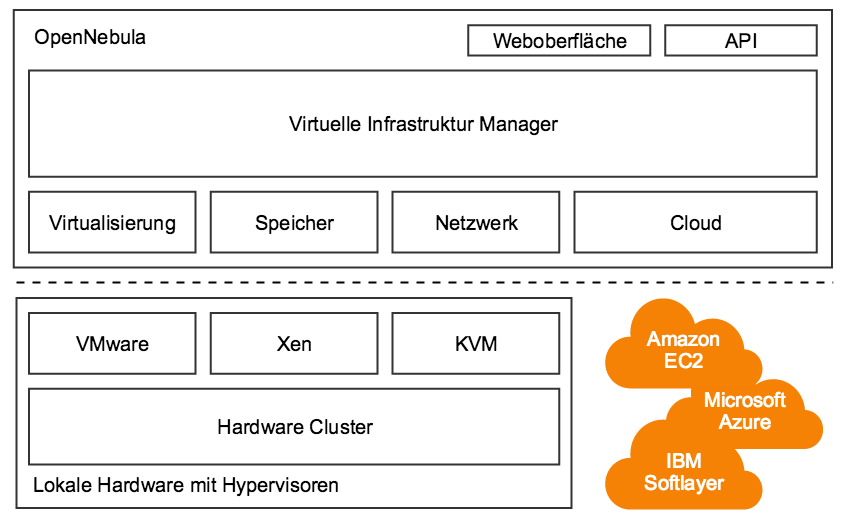
\includegraphics[width=0.99\textwidth]{img/opennebula.png}
	\caption[Architektur von OpenNebula, apatiert aus \cite{molina2012}]{Grundlegende Architektur von OpenNebula. Die strichlierte Linie zeigt die Trennung zwischen OpenNebula und der verwalteten Hardware. Apatiert aus \cite{molina2012}}
	\label{fig:opennebula_architecture}
\end{figure} 

Ein weiterer Vorteil von OpenNebula ist, dass neben lokaler Hardware auch gängige Cloud Services (siehe Abbildung \ref{fig:opennebula_architecture}) wie Amazon EC2, Microsoft Azure oder IBM Softlayer als Infrastruktur für virtuelle Maschinen genutzt werden können. Somit können mehrere Infrastrukturen über dasselbe System verwaltet werden. Weiters ist es möglich Rechte für die Verwaltung einzelner virtueller Maschinen an Benutzer zu koppeln. Somit können die einzelnen Umgebungen auch mit unterschiedlichen Rechten getrennt werden, um mögliche Fehler durch Verwechslungen zu verhindern \cite{molina2012}.

\subsection{Agiles Entwicklungsmodell}
DevOps und Continuous Delivery versuchen die Konzepte und Vorteile von agilen Entwicklungsmethoden auf den Software-Betrieb anzuwenden. Aus diesem Grund können die Vorteile von DevOps ebenfalls nur dann entsprechend zur Geltung kommen, wenn auch die Entwicklung bereits nach agilen Methoden vorgeht. Vor allem, wenn zusätzlich zu DevOps noch Continuous Delivery erreicht werden soll, sind agile Entwicklungsmodelle unumgänglich. Ansonsten kann im Betrieb schnell auf Anforderungen reagiert werden, aber die Entwicklung verzögert den Vorgang. Es müssen also die Software-Entwicklung \textbf{und} der Betrieb nach agilen Vorgehensmodellen arbeiten. Die Red Bull Media Base entwickelt seit Beginn 2013 jede Applikation nach dem Kanban Prinzip. Die meisten Projekte veröffentlichen neue Versionen in einem regelmäßigen Abstand von zwei Wochen \cite{gluchowski2013}.

\section{Ausgewählte Systeme und Konzepte}
\label{sec:systemeundkonzepte}
Wie im theoretischen Teil erwähnt, behandelt der technische Aspekt von DevOps die Automatisierung von Aufgaben. Häufig auftretende Tätigkeiten wie Software bauen, testen und deployen sollen nicht mehr manuell durchgeführt werden. Für die Automatisierung dieser Tätigkeiten werden entsprechende Systeme benötigt. Eine große Anzahl an Beispielen für Systeme unterschiedlicher Aufgaben sind in \cite{skelton2014} gelistet. In den nachfolgenden Abschnitten werden die vom Projektteam gewählten Systeme, sowie die entwickelten Konzepte, beschrieben. Je Abschnitt wird das vorhandene Problem erläutert und wie dieses mit dem gewählten System/Konzept gelöst wird.

\subsection{Konfigurationsmanagement mit Ansible}
Das Konfigurationsmanagement stellt einen zentralen Bestandteil von DevOps dar. Damit wird die Infrastruktur nachvollziehbar und reproduzierbar definiert. Es unterstützt die Automatisierung und eliminiert folglich manuelle Tätigkeiten. Bisher wurde im Umfeld der Red Bull Media Base kein Konfigurationsmanagemensystem genutzt. 

Für das Konfigurationsmanagement und die Orchestrierung der Infrastruktur gibt es unzählige Systeme auf dem Markt \cite{skelton2014}. Viele davon, wie etwa Puppet\footnote{\url{https://puppetlabs.com/about/customers}, u.a. Cisco, Intel, NASA und Spotify} oder Chef\footnote{\url{https://www.chef.io/customers/}, u.a. Etsy, Rackspace und Facebook}, werden laut eigenen Angaben von vielen namhaften Unternehmen verwendet. Eine Evaluierung dieser Systeme ergab aber einen entscheidenden Nachteil für die Red Bull Media Base. Puppet sowie Chef verfolgen eine Client-Server Architektur der Infrastruktur. Ein zentraler Server verwaltet die Konfiguration der Clients und sendet diese regelmäßig an die Clients. Dafür muss aber auf jeder Maschine der entsprechende Client installiert und konfiguriert sein \cite{pandey2012}. Bevor man mit dem Deployment der Software beginnen kann, müssen somit noch zusätzliche Tätigkeiten, nach der Erstellung der Maschine, durchgeführt werden. Daher wurde nach einer clientlosen Alternative gesucht. Ansible stellte sich als eine Alternative heraus.

\paragraph{Kriterien für die Wahl von Ansible:}
Ansible ist ein Konfigurationsmanagement System auf Basis von Python, das keine Clients auf den Maschinen benötigt. Voraussetzungen für Ansible sind lediglich eine SSH Verbindung zur Maschine und eine Python Umgebung mit minimaler Version 2.6. Da Python grundsätzlich Bestandteil von Linux Distributionen ist, sind diese Voraussetzungen gegeben \cite{ansible2014, hall2013}.

Die Vorteile der clientlosen Architektur von Ansible sind laut \cite{ansible2014} folgende und haben maßgeblich zu dessen Auswahl beigetragen:
\begin{itemize}
	\item Zwischen der Maschine die Ansible ausführt und der Zielmaschine werden nur Python Skripte und deren Ergebnisse ausgetauscht. Es erfolgt keine weitere Kommunikation und beschränkt den Netzwerkverkehr auf ein Minimum.
	\item Ansible bietet hohe Sicherheit, da die ausgereifte Implementierung von OpenSSH genutzt und keine eigene Verschlüsselung und Transportsicherung entwickelt wird.
	\item Da es keinen zentralen Konfigurationsserver gibt, können Clients auch keine kritischen Daten/Konfigurationen (z.B. Passwort-Dateien) anderer Maschinen abfragen. Ansible transferiert nur die unbedingt benötigten Daten auf eine Maschine. Eine kompromittierte Maschine kann daher keine anderen Daten abfragen.
	\item Die Verwaltung des Konfigurationsservers entfällt und es muss nicht darauf geachtet werden, dass die Version von Server und Client zusammenpassen. Updates von Ansible müssen lediglich auf der ausführenden Maschine abgewickelt werden.
	\item Es gibt keine Skalierungsprobleme bei Ansible, da die Clients nicht ständig von einer zentralen Instanz überprüft werden. Die tatsächlichen Aufgaben werden direkt von der Zielmaschine ausgeführt und nicht von einem zentralen Server. Damit verteilt sich die komplette Last über alle Maschinen.
	\item Da kein Client benötigt wird, verbraucht dieser auch keine Ressourcen auf der Zielmaschine. Es wird nur Last erzeugt, wenn konkrete Aufgaben durchgeführt werden und nicht durch regelmäßige Checks.
	\item Die Deklarationen werden im YAML Format verfasst und daher für Entwickler leicht lesbar. Da auch immer nur der gewünschte Endzustand beschrieben wird, und nicht die nötigen Schritte um dortin zu gelangen, kann schnell erfasst werden, welche Konfiguration angewandt wird. 
\end{itemize}

Ein Nachteil von Ansible, gegenüber Systemen mit zentralem Server ist, dass Konfigurationen nicht ständig erzwungen werden. Bei einem zentralen System werden  manuell durchgeführte Änderungen auf einer Maschine beim nächsten Check wieder entfernt. Die lokale Konfiguration wird ständig mit der zentralen Konfiguration abgeglichen. Bei Ansible werden manuelle Änderungen nur bei erneuter Provisionierung der Maschine entfernt. Ein weiterer Nachteil ist, dass Ansible aktuell nur sehr wenig Unterstützung für Windows bietet. Da die Red Bull Media Base aber aktuell keine Windows Server einsetzt, ist dieser Nachteil nicht relevant. Bei Ansible überwiegen im konkreten Bedarf die Vorteile gegenüben den Nachteilen, weswegen sich das Projektteam für den Einsatz von Ansible entschieden hat \cite{hall2013}.

\paragraph{Grundsätzliche Funktionsweise von Ansible:} 
Ähnlich wie bei Chef/Puppet wird bei Ansible der gewünschte Endzustand einer Maschine beschrieben. Dies geschieht in der Sprache YAML\footnote{\url{http://www.yaml.org/spec/1.2/spec.html}, YAML Ain’t Markup Language}. Die Summe aller Deklarationen wird Playbook genannt. Führt man ein Playbook aus, so werden alle nötigen Schritte unternommen, um den darin definierten Zustand zu erreichen. Auflistung \ref{lst:ansible:playbook} zeigt als Beispiel das Playbook der Delivery Agent Applikation aus Abschnitt \ref{sec:deliveryagent}.

\begin{lstlisting}[style=code,numbers=left,caption={Beispiel: Ansible Playbook des Delivery Agents},label={lst:ansible:playbook}]
- hosts: da-application
  sudo: yes
  vars:
    umgebung: "{{lookup('env','ONE_INVENTORY_ENV')}}"
    sensu_server_rabbitmq_hostname: sensu.rbmbtnx.net
    logstash_server: logstash.rbmbtnx.net
  pre_tasks:
    - name: load variables for the particular environment
      include_vars: "{{item}}"
      with_items:
        - "../aux_vars/all/main.yml"
        - "../aux_vars/da/{{umgebung}}.yml"
  roles:
    - {role: rbmh.common, tags: 'common'}
    - {role: rbmh.delivery-agent.ha, tags: 'deployment'}
    - {role: rbmh.logstash-shipper}
    - {role: rbmh.sensu-client}
  tasks:
    - name: register public service url with dns
      uri: url="https://{{ip_dns_vip}}/api/add_zone.php?name={{public_service_uri}}&ext={{keepalived_shared_ip}}&int={{keepalived_shared_ip}}&typ=nosite&id=8dfk38sdERe8sdA923n" 
      run_once: true
\end{lstlisting}

Für eine bessere Gliederung der einzelnen Zustände von Komponenten, können diese in Pakete namens Roles unterteilt werden. Somit kann ein Playbook als eine Menge von Roles angesehen werden, die wiederum aus einer Vielzahl an Tasks bestehen. In diesem Fall werden Roles für die Installation der Delivery Agent Applikation, des Sensu Clients (Abschnitt \ref{sec:sensu_client}) und der Log-Lieferung (Abschnitt \ref{sec:logstash:shipper}) durchgeführt. Wie \autoref{lst:ansible:playbook} zu entnehmen, können auch noch zusätzliche Tasks angegeben werden.

Aus den Deklarationen generiert Ansible Python Skripte (sogenannte Module), die auf die Maschinen transferiert und dort ausgeführt werden. Module erkennen automatisch, welche Schritte nötig sind, um den gewünschten Zustand zu erreichen. Ist dieser Zustand bereits vorhanden, so werden keine Schritte vollzogen. Egal wie oft man eine Aufgabe durchführt, der Endzustand ist immer der Gleiche. Dieses Verhalten nennt man \textit{Idempotent} \cite{hall2013}.

Die zweite Komponente zu den Playbooks ist das sogenannte Inventory. Playbooks geben an, welcher Zustand erreicht werden soll und das Inventory, auf welchen Maschinen dieser Zustand gewünscht ist. Es beinhaltet die Liste aller Maschinen, aufgeteilt in Gruppen \cite{hall2013}. Im Playbook wird an der Stelle \textit{hosts: da-application} angegeben, dass es nur für die Maschinen der Gruppe \textit{da-application} gültig ist. Ein Inventory kann in zwei Formaten angegeben werden. Entweder im INI-Format oder als JSON. Auflistung \ref{lst:ansible:inventory} zeigt beide Möglichkeiten für drei Maschinen des Delivery Agents.

\begin{lstlisting}[style=code,numbers=left,caption={Beispiele: Ansible Inventory des Delivery Agent},label={lst:ansible:inventory}]
"da-application": {
   "hosts": [
      "172.20.35.84",
      "172.20.35.85",
      "172.20.35.86",
   ]
}
---------------------
[da-application]
172.20.35.84
172.20.35.85
172.20.35.86
\end{lstlisting}


\paragraph{Einsatz bei der Red Bull Media Base:}
Quellcode sollte möglichst wiederverwendbar geschrieben werden, um zukünftige Aufwände zu reduzieren. Daher wird der Aufgabenbereich einer Ansible Role so aufgeteilt, dass sie jeweils für die Installation einer Komponente zuständig ist. So ergeben sich beispielsweise Roles für die Installation von Java, oder des Tomcat Webservers. Dadurch können die Roles bei jedem Service, das eine entsprechende Komponente benötigt, wiederverwendet werden. Dieser Ansatz ist von entscheidender Bedeutung und reduziert den nötigen Aufwand der Implementierung drastisch. Ein weiterer Vorteil ist, dass die Komponente auf allen Maschinen gleich installiert ist. Unterschiedliche Arten von Installationen sind nicht möglich und daher wird der Verwaltungsaufwand reduziert. Die spezielle Konfiguration der Komponenten erfolgt danach in einer Role für die jeweilige Applikation. Sind die Aufgabenbereiche der einzelnen Roles voneinander abgegrenzt, so besteht ein Playbook grundsätzlich nur mehr aus der Kombination der Roles für die Installation der benötigten Komponenten, plus eine Role für die Applikation selbst, wie in \autoref{lst:ansible:playbook} zu sehen ist.

Außerdem sind alle umgebungsspezifischen Konfigurationen als Variablen ausgegliedert. Somit wird dieselbe Role für die Installation in allen vier Umgebungen verwendet. Die spezifischen Variablen für die jeweilige Umgebung werden zu Beginn des Playbook, wie in \autoref{lst:ansible:playbook} in Zeile 10, geladen. Dies gilt ebenso für die lokale Entwicklungsumgebung. In den folgenden Abschnitten wird bei den Metriken immer auf die Anzahl der Roles verwiesen, die wiederverwendet wurden. Dieser Aufwand entfällt somit für die jeweilige Applikation.

Durch die Möglichkeit, das Inventory in JSON angeben zu können, ist es möglich, Ansible mit OpenNebula zu kombinieren. Über die API von OpenNebula kann die Liste der aktuell verfügbaren Maschinen abgerufen werden. Diese Liste wird in ein JSON Format umgewandelt und anhand von Metadaten an den Maschinen die Gruppen erstellt. Somit ist immer ein aktuelles Inventory für Ansible verfügbar und muss nicht manuelle gepflegt werden.

\paragraph{Erfassen der Metriken:}
Da Ansible für die Provisionierung zuständig ist, können die Metriken der Durchlaufzeit für Ansible nicht erfasst werden. In Tabelle \ref{tab:metric:ansible} sind daher nur die Aufwände für die Konzeption der Struktur der Roles, das Einlernen des Projektteams und die Installation von Ansible auf einer Maschine aufgeführt.

\begin{table}[ht]
%\setlength{\arrayrulewidth}{0.3mm}
\setlength{\tabcolsep}{5pt}
\renewcommand{\arraystretch}{1.5}
\centering
\begin{tabular}{|l|l|l|}
\hline
\rowcolor[HTML]{C0C0C0}
\multicolumn{2}{|c|}{\textbf{Metrik}} 				& \textbf{Menge}		\\ 
\hline
\multirow{3}{*}{Initialer Aufwand}	& Konzeption 	& 24 PS			\\ 
\cline{2-3}
									& Einlernen		& 100 PS			\\			\cline{2-3}
									& Installation 	& 0.5 PS 		\\
\hline
\end{tabular} 
\caption{Erfasste Metriken für Ansible}
\label{tab:metric:ansible}
\end{table}

Die Konzeption der Struktur der einzelnen Elemente von Ansible und ein Machbarkeitstest beanspruchte etwa drei Arbeitstage. Dies wurde von Alexander Dobriakov durchgeführt, da er bereits Erfahrung mit Ansible aufweisen konnte. Die restlichen Projektmitglieder mussten sich erst mit Ansible vertraut machen. Das Einlernen in Ansible erstreckte sich auf mehr als eine Arbeitswoche pro Person. Anschließend war genug Wissen vorhanden, um die meisten Aufgaben durchzuführen. Die Installation von Ansible war in wenigen Minuten abgeschlossen, da es via pip\footnote{\url{http://docs.ansible.com/intro_installation.html\#latest-releases-via-pip}, Installationsanleitung der offiziellen Dokumentation} verfügbar ist.

\subsection{Build und Deployment Pipeline mit Bamboo}
\label{sec:pipeline}
In vielen Software Unternehmen wird bereits Continuous Integration (CI) betrieben, um möglichst schnell Änderungen in die Software zu integrieren. Somit bekommen die Entwickler schneller Feedback, ob die Software nach den Änderungen noch gebaut werden kann. Diese Aufgabe wird meist von einem sogenannten Build-Server durchgeführt \cite{wolff2014}. Die Red Bull Media Base verwendet als Build und Deployment Server \textit{Bamboo}\footnote{\url{https://de.atlassian.com/software/bamboo}, kommerzielles Produkt von Atlassian}. In der Vergangenheit wurde Jenkins\footnote{\url{https://wiki.jenkins-ci.org/display/JENKINS/Meet+Jenkins}, OpenSource Build Server} verwendet, allerdings bietet dieser nur über Community Plugins die Möglichkeit, Deployments zu verwalten. Die Integration der Plugins funktioniert allerdings nicht immer einwandfrei. Daher wurde entschieden, bei diesem zentralen Bestandteil auf kommerzielle Software zu setzen. 

\paragraph{Einsatz bei der Red Bull Media Base:} Bamboo stellt den zentralen Bestandteil der gesamten DevOps Infrastruktur dar. Es ist bei allen Projekten für den Build der Software Artefakte und die Verwaltung der Deployments zuständig. Diese Maschine muss somit Zugriff auf alle anderen Maschinen im DC2.0 haben. Daher ist Bamboo eine der wenigen Maschinen die im ADMIN Subnetz des DC2.0 angesiedelt ist.

Für die Verwaltung der Builds und Deployments gibt es in Bamboo zwei Konzepte namens \textit{Build- und Deploymentpläne}. Für jedes Software-Projekt wird ein Buildplan konfiguriert. Dieser führt automatisch die nötigen Schritte aus und erzeugt Artefakte für die neueste Applikationsversion. Anschließend werden Unit-Tests ausgeführt und ausgewertet. Der Build ist nur dann erfolgreich abgeschlossen, wenn diese keinen Fehler melden. Die erzeugten Artefakte werden anschließend in einem Artefakt Repository (siehe \ref{sec:tools:sonstige}) gespeichert. 
Da der Quellcode der Projekte mit Git verwaltet wird, überwacht Bamboo die Repositories auf neue Commits. Werden Änderungen eingecheckt so startet Bamboo automatisch den Build um Continuous Integration zu betreiben.

Mittels Deploymentplänen werden die Deployments auf die einzelnen Maschinen gesteuert und verwaltet. In Bamboo ist es möglich, pro Projekt mehrere Umgebungen zu verwalten und demnach die im Media Base Umfeld existierenden vier Umgebungen abzubilden. Für die Provisionierung der Software, werden bei jedem Deploymentplan entsprechende Ansible Playbooks hinterlegt. Wird nun ein Deployment durchgeführt, so startet Bamboo das hinterlegte Playbook und markiert die Umgebung als OK, sofern dieses keinen Fehler liefert. Es ist außerdem möglich, Deploymentpläne an die dazugehörigen Buildpläne zu koppeln. Sobald ein erfolgreicher Build stattgefunden hat, wird der Deploymentplan automatisch ausgeführt und somit Continuous Delivery erreicht. Dies wird aber aktuell noch bei keinem Projekt verwendet. Die Deploymentpläne werden alle manuell ausgeführt.

\paragraph{Versionsverwaltung der Ansible Playbooks:} Die genauen Schritte eines Deployments sind in den Playbooks definiert. Um ein Deployment jederzeit nachvollziehen zu können, muss der aktuelle Stand der Playbooks, zum Zeitpunkt des Deployments, erfasst werden. Ansonsten ist es möglich, unterschiedliche Versionen der Playbooks für dasselbe Deployment in unterschiedlichen Umgebungen zu verwenden. Dies kann zu schwer nachvollziehbaren Fehlern führen. Um die Version der Playbooks festzuhalten, wurde ein eigener Buildplan eingerichtet. Dieser testet die aktuellsten Playbooks auf syntaktische Korrektheit und speichert diese Version als eigenes Artefakt mit laufender Nummer ab. Im Deploymentplan eines Projekts kann gewählt werden, welche Version für das Deployment verwendet wird.

\begin{figure}[ht]
	\centering
	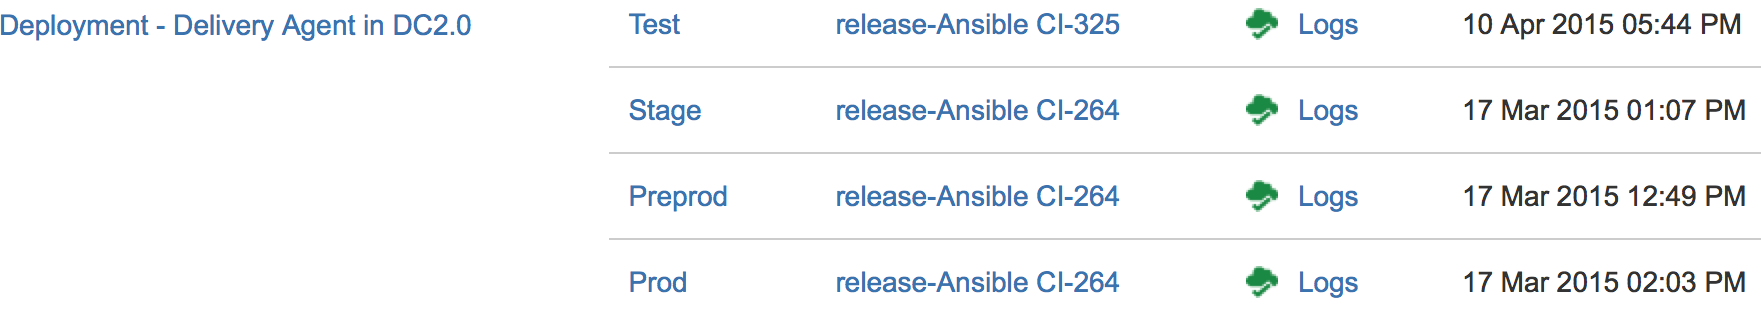
\includegraphics[width=0.99\textwidth]{img/da_deployment.png}
	\caption[Deploymentplan des Delivery Agent]{Der Deyplomentplan des Delivery Agent. Die verwendete Version der Playbooks ist direkt an der Umgebung ersichtlich. Somit wird ein hohes Maß an Nachvollziehbarkeit erreicht.}
	\label{fig:deployment:da}
\end{figure} 

\autoref{fig:deployment:da} zeigt den Deploymentplan des Delivery Agent. Die Version der Playbooks, die verwendet wurde um die Applikation in einer bestimmten Umgebung zu deployen, ist sofort ersichtlich. In diesem Beispiel erkennt man, dass Staging, PreProduktion und Produktion aktuell denselben Stand aufweisen, \textit{CI-264}. In der Testumgebung wurde bereits eine neuere Version deployed, \textit{CI-325}. Zusätzlich wird angezeigt, ob das letzte Deployment korrekt verlaufen ist und wann es durchgeführt wurde.

\paragraph{Erfassen der Metriken:} \autoref{tab:metric:bamboo} listet die Metriken für die Aufwände der Installation von Bamboo, sowie die Durchlaufzeit für ein Update auf.
\begin{table}[ht]
%\setlength{\arrayrulewidth}{0.3mm}
\setlength{\tabcolsep}{5pt}
\renewcommand{\arraystretch}{1.5}
\centering
\begin{tabular}{|l|l|l|}
\hline
\rowcolor[HTML]{C0C0C0}
\multicolumn{2}{|c|}{\textbf{Metrik}} 				& \textbf{Menge}		\\ 
\hline
\multirow{3}{*}{Initialer Aufwand}	& Installation von Bamboo & 40 PS	\\ 
\cline{2-3}
									& Basiskonfiguration 	 & 4 PS		\\
\cline{2-3}
									& Konfiguration je Projekt & 1 PS	\\
\hline
Durchlaufzeit				 		& Update	 von Bamboo		& ca. 15 Minuten		\\ 
\hline
\end{tabular}
\caption{Erfasste Metriken für Bamboo}
\label{tab:metric:bamboo}
\end{table}
Da die Installation von Bamboo und aller benötigten Komponenten mit Ansible durchgeführt wird, ist der initiale Aufwand höher als bei einer manuellen Installation. Dadurch können Updates von Bamboo über Ansible durchgeführt werden, das wiederum weniger Zeit erfordert, gegenüber manuell durchgeführten Updates. Die Basiskonfiguration von Bamboo beinhaltet allgemeinen Dinge, die nur einmal für alle Projekte notwendig sind. Je Software-Projekt muss wie erwähnt ein Build- und Deploymentplan erstellt werden. Dies dauert jeweils etwa eine Personenstunde.

\subsection{Lokale Entwicklungsumgebung mit Vagrant}
Beim Betrieb einer Applikation wird meist nur auf die Umgebungen im Rechenzentrum geachtet, nicht aber auf die lokale Entwicklung. So wird lokal unter anderen Voraussetzungen entwickelt, als die Applikation später im Rechenzentrum läuft. Dies macht das lokale Testen ineffizient und führt zu unentdeckten Fehlern. Um dem entgegen zu wirken, wird eine Kombination aus Vagrant\footnote{\url{http://docs.vagrantup.com/v2/why-vagrant/}, leichtgewichtige Virtualisierungsumgebung} und Ansible eingesetzt. Mit Vagrant lassen sich virtuelle Umgebungen in textueller Form definieren, was diese leicht reproduzierbar und portierbar macht. So ist sichergestellt, dass die Entwickler immer dieselbe virtuelle Infrastruktur für die lokale Entwicklung nutzen. Bei der Erstellung der virtuellen Umgebung können außerdem Provisionierungsprozesse mit Ansible angestoßen werden, um die benötigte Software in der virtuellen Umgebung zu installieren. Da hier dieselben Ansible Playbooks wie in Produktion verwendet werden, ist diese Umgebung sehr nahe an der produktiven Umgebung. Ganze Cluster können ohne erheblichen Aufwand aufgebaut werden, um solche Szenarien in der Entwicklung zu simulieren. Obwohl sich nicht alle Unterschiede beseitigen lassen, steigt dennoch die Effizienz bei der Entwicklung erheblich.
 
\begin{lstlisting}[style=code,numbers=left,caption={Beispielhaftes Vagrantfile des Delivery Agent},label={lst:vagrantfile}]
Vagrant.configure(2) do |config|
  config.vm.box = "centos-6.6-x86_64"
  config.vm.box_url = "https://repo.rbmb.com/vagrant/centos66.json"
  
  config.vm.define :web1 do |web1_config|
    web1_config.vm.hostname = "web1.da.vagrant"
    web1_config.vm.provider "virtualbox" do |vb|
      vb.customize ["modifyvm", :id, "--name", "web1.da.vagrant", "--memory", "512", "--cpus", "1", "--ioapic", "on"]
    end
    web1_config.vm.network "private_network", ip: "192.168.33.101"
    web1_config.vm.provision "ansible" do |ansible|
      ansible.playbook = "test.yml"
      ansible.inventory_path = "vagrant_servers"
      ansible.limit = "da-application"
    end
  end

  # VM Konfiguration der Loadbalancer Node
  config.vm.define :lb1 do |lb_config|
    lb_config.vm.hostname = 'lb1.da.vagrant'
    lb_config.vm.provider "virtualbox" do |vb|
      vb.customize ["modifyvm", :id, "--name", "lb1.da.vagrant", "--memory", "256", "--cpus", "1", "--ioapic", "on"]
    end
    lb_config.vm.network "private_network", ip: "192.168.33.103"
    lb_config.vm.provision "ansible" do |ansible|
      ansible.playbook = "lb.yml"
      ansible.inventory_path = "vagrant_servers"
      ansible.limit = "lbh-service"
    end
  end
end
\end{lstlisting}

Die virtuelle Umgebung wird in einem sogenannten \textit{Vagrantfile} definiert. \autoref{lst:vagrantfile} zeigt das Vagrantfile des Delivery Agent. Zuerst werden allgemeine Definitionen der Umgebung angegeben, wie beispielsweise das Betriebssystem für die virtuellen Maschinen (Zeilen 2 und 3). Anschließend wird eine Node für den Delivery Agent, sowie eine Loadbalancer Node definiert. Je Node wird der Hostname, RAM, CPU und die IP-Adresse angegeben. Für jede Node ist angegeben, welches Playbook und Inventory für Ansible verwendet werden soll (Zeilen 11-14 bzw. 25-28). Die Provisionierung wird durchgeführt, sobald die virtuellen Maschinen verfügbar sind.

\begin{table}[ht]
%\setlength{\arrayrulewidth}{0.3mm}
\setlength{\tabcolsep}{5pt}
\renewcommand{\arraystretch}{1.5}
\centering
\begin{tabular}{|l|l|l|}
\hline
\rowcolor[HTML]{C0C0C0}
\multicolumn{2}{|c|}{\textbf{Metrik}} 			& \textbf{Menge}		\\ 
\hline
Initialer Aufwand			& Installation von Vagrant	& 0.5 PS		\\ 
\hline
\end{tabular}
\caption{Erfasste Metriken für Vagrant}
\label{tab:metric:vagrant}
\end{table}

Vagrant bietet jedoch keine Virtualisierung und benötigt eine bereits vorhandene Virtualisierungsumgebung, wie etwa Virtualbox. Dies wird als \textit{Provider} bezeichnet und ebenfalls im Vagrantfile angegeben (Zeile 7 bzw. 21). Vagrant ist für alle Betriebssysteme verfügbar und lässt sich innerhalb einer halben Stunde installieren (\autoref{tab:metric:vagrant}). Eine spezielle Konfiguration ist nicht erforderlich. Die Installation muss allerdings auf jedem Entwicklungsrechner durchgeführt werden.

\subsection{Lifecycle der Applikationen im DC2.0}
\label{sec:lifecycle}
Die Konzepte von DevOps müssen nicht nur im Betrieb, sondern bereits in der Entwicklung beachtet werden. Die Applikationen selbst müssen nach gewissen Vorgaben adaptiert werden, um sie entsprechend betreiben zu können. Die nachfolgende Liste erklärt generelle Schritte, die je Applikation umgesetzt werden müssen. Diese Definitionen garantieren, dass eine Applikation mit den Konzepten des DC2.0 konform ist und deshalb auch betrieben werden kann. 

\begin{enumerate}
	\item Der Build der Applikation muss mit Gradle durchgeführt, und über Buildpläne in Bamboo verwaltet werden. Resultierende Artefakte müssen im Artefakt Repository gespeichert werden. So wird die Reproduzierbarkeit der Artefakte sichergestellt. Alle Projekte der Red Bull Media Base werden bereits mit Gradle gebaut. Daher müssen nur mehr die entsprechenden Buildpläne in Bamboo erstellt werden.
	\item Die Erstellung der virtuellen Maschine und die Installation aller Applikationen müssen mit Ansible durchgeführt werden. Dies gilt auch für jegliche Konfigurationsänderung. Es dürfen keinerlei manuellen Tätigkeiten mehr notwendig sein, um die Applikation zu installieren und zu konfigurieren. 
	\item Die Provisionierung der Software in den verschiedenen Umgebungen muss mit denselben Playbooks durchgeführt werden. Unterschiede zwischen den einzelnen Umgebungen müssen als Variablen definiert sein.
	\item Eine entsprechende Dokumentation muss für ein Projekt vorhanden sein. Diese Dokumentation muss Informationen über Kontrollprozeduren, Notfallmaßnahmen, Monitoring und Backup enthalten. Ohne Dokumentation kann keine Verfügbarkeit für die Applikation im DC2.0 garantiert werden.
	\item Bei neuen Projekten muss geprüft werden, ob die generellen Netzwerkregeln (Abschnitt \ref{sec:netzwerk}) ausreichend sind oder ob eine Erweiterung notwendig ist.
	\item Um ausreichende Monitoring Checks durchführen zu können, muss die Applikation zwei Diagnose-Endpunkte (/health und /metrics) anbietet. Der Endpunkt /health muss die Information beinhalten, ob die Applikation operativ ist oder ob es Fehler gibt. Der Endpunkt /metrics muss sinnvolle Metriken anführen, wie beispielsweise die aktuelle Last oder Anzahl der offenen Verbindungen.
	\item Als Logging Framework soll logback\footnote{\url{http://logback.qos.ch}, Logging Framework für Java} verwendet werden, da somit eine einfache Integration von Logstash (Abschnitt \ref{sec:logstash:main}) möglich ist.
	\item Die virtuellen Maschinen für die Applikation müssen über eine Formation (Abschnitt \ref{sec:formation}) erstellt werden. Es darf keine virtuelle Maschine geben, die manuell erstellt wurde. Das garantiert die Reproduzierbarkeit der Maschinen im DC2.0.
	\item In Bamboo muss ein Deploymentplan angelegt werden. Bei Applikationen die aus einem Cluster mit mehreren Nodes bestehen, muss das Deployment mit dem Zusatz \textit{serial: 1} ausgeführt werden. Dies garantiert, dass Ansible immer nur eine Node zur gleichen Zeit provisioniert und es somit zu keinem Ausfall kommt.
	\item Applikationen die über das Internet erreichbar sein sollen, müssen in den Loadbalancer (Abschnitt \ref{sec:loadbalancer}) integriert werden. Dafür müssen sich die einzelnen Maschinen über Consul beim Loadbalancer registrieren.
	\item Direkt nach der Installation der Applikation müssen sogenannte Smoke-Tests durchgeführt werden, um die grundsätzliche Verfügbarkeit und korrekte Arbeitsweise zu garantieren.
\end{enumerate}

Nach Durchführung dieser Schritte ist die Applikation bereit für den Betrieb im DC2.0. Weiters garantieren sie, dass jederzeit ein lauffähiger Zustand der Applikation, innerhalb einer kurzen Dauer, wiederhergestellt werden kann.

\paragraph{Erfassen der Metriken:}
Der initiale Aufwand für das Konzept des Lifecycle kann nur schwer erfasst werden. Der Lifecycle hat sich aus den Rahmenbedingungen ergeben, die mit der Basisinfrastruktur einhergehen und wurde nicht explizit als Erstes erstellt. Er wurde nachträglich als Richtlinie für die Applikationen definiert, um den Prozess zu formalisieren. Der Aufwand in der \autoref{tab:metric:lifecycle} bezieht sich also nur auf die Formalisierung des Lifecycle unter Absprache der Projektmitglieder.

\begin{table}[ht]
%\setlength{\arrayrulewidth}{0.3mm}
\setlength{\tabcolsep}{5pt}
\renewcommand{\arraystretch}{1.5}
\centering
\begin{tabular}{|l|l|l|}
\hline
\rowcolor[HTML]{C0C0C0}
\multicolumn{2}{|c|}{\textbf{Metrik}} 		& \textbf{Menge}		\\ 
\hline
Initialer Aufwand			& Konzeption	 \& Formalisierung 	& 15 PS				\\ 
\hline
\end{tabular}
\caption{Erfasste Metriken für den Lifecycle}
\label{tab:metric:lifecycle}
\end{table}

Würde der Lifecylce als Erstes erstellt, so würde der Aufwand entsprechend höher ausfallen. Allerdings muss für diese Vorgehensweise ein hohes Maß an Erfahrung vorhanden sein. Ansonsten würde sich die Definition des Lifecylce im Laufe der Implementierung, aller Voraussicht nach, mehrmals verändern.

\subsection{Erstellung von virtuellen Maschinen}
\label{sec:formation}
Die Automatisierung der Prozesse umfasst möglichst alle Bereiche des Betriebs. Oftmals wird die Erstellung der virtuellen Maschinen nicht berücksichtigt. Sie werden noch manuell erstellt und anschließend in die Automatisierungsprozesse eingebunden. Diese Vorgehensweise hat zur Folge, dass die Maschinen nicht reproduzierbar sind. Wird eine neue Maschine hinzugefügt, so ist nicht festgehalten wie die genaue Konfiguration lautet. Daher kann es zu unterschiedlichen Konfiguration kommen, was wiederum zu schwer nachvollziehbaren Fehler führen kann.

\paragraph{Einsatz bei der Red Bull Media Base:} 
Um dieses Problem zu bewältigen, setzt die Red Bull Media Base sogenannte Formation Skripte\footnote{Der Name ist in Anlehnung and die CloudFormation von Amazon} ein. Durch seine API ermöglicht OpenNebula die automatisierte Erstellung von virtuellen Maschinen. Dazu muss der API die Definition der Maschine in einem strukturierten Format übergeben werden. Das ermöglicht, die Maschinen für eine Applikation als Template zu definieren und sie nachvollziehbar festzuhalten. Die Templates werden von Ansible verwendet und die Variable im Template bei der Ausführung ersetzt. Ansible übergibt das ausgefüllte Template der API von OpenNebula und erstellt die Maschine. Durch die Verwendung dieser Templates entsteht jedes mal dieselbe virtuelle Maschine. Unterschiede zwischen den Maschinen werden verhindert und Fehler dieser Art können ausgeschlossen werden. Die \autoref{lst:formation:template} zeigt ein Beispiel für ein Template. 

\begin{lstlisting}[style=code,numbers=left,caption={Beispiel eines Formation Template für virtuelle Maschinen},label={lst:formation:template}]
NAME="{{vm_name}}"
CONTEXT=[
    SET_HOSTNAME="$NAME.$NETWORK[FUNCTIONAL_NAME,NETWORK=\"{{primary_network}}\"].{{datacenter}}.rbmbtnx.net",
    SSH_PUBLIC_KEY="$USER[SSH_PUBLIC_KEY]",
    NETWORK="YES"
]
HYPERVISOR="kvm"
DISK=[IMAGE="centos-7.1.0",IMAGE_UNAME="opennebula-test"]
DISK=[DRIVER="qcow2",SIZE="100000",TYPE="fs",FORMAT="qcow2"]
NIC=[NETWORK_UNAME="oneadmin",NETWORK="{{primary_network}}"]
MEMORY="4096"
CPU="0.02"
VCPU="2"
SCHED_REQUIREMENTS="ID=\"12\""

# Red Bull spezifische Variablen
DATACENTER="{{datacenter}}"
UMGEBUNG="{{umgebung}}"
LAYER="{{layer}}"
STACK="{{service}}"
\end{lstlisting}
In diesem Template werden Konfigurationen, wie der verwendete Hypervisor (Zeile 7), die Netzwerkschnittstellen (Zeile 10), der verfügbare RAM \& CPU (Zeilen 11-13), zusätzliche Festplatten (Zeile 9) und das Basisimage (Zeile 8) für die virtuelle Maschine festgehalten. Außerdem können an einer Maschine beliebige Variablen gespeichert werden (ab Zeile 16), die man wiederum in Ansible Playbooks nutzen kann. 

\paragraph{Erfassen der Metriken:}
Für die Konzeption der Formation Skripte musste die API von OpenNebula und die Struktur der Templates verstanden werden. Da jede Applikation meist unterschiedlich konfigurierte Maschinen erfordert, müssen die Formation Skripte pro Applikation erstellt werden. Meist sind nur leichte Anpassungen nötig, weswegen bereits erstellte Formation Skripte wiederverwendet werden können.

\begin{table}[ht]
%\setlength{\arrayrulewidth}{0.3mm}
\setlength{\tabcolsep}{5pt}
\renewcommand{\arraystretch}{1.5}
\centering
\begin{tabular}{|l|l|l|}
\hline
\rowcolor[HTML]{C0C0C0}
\multicolumn{2}{|c|}{\textbf{Metrik}} 		& \textbf{Menge}		\\ 
\hline
\multirow{2}{*}{Initialer Aufwand}			& Konzeption		& 24 PS	\\ 
\cline{2-3}
											& je Projekt 	& 2 PS	\\
\hline
Durchlaufzeit				& erstellen einer Maschine  & ca. 5-10 Minuten \\ 
\hline
\end{tabular}
\caption{Erfasste Metriken für Formation Skripte}
\label{tab:metric:formation}
\end{table}

Die Durchlaufzeit in \autoref{tab:metric:formation} bezeichnet die Zeit die benötigt wird, bis eine Maschine für die Installation der Komponenten einsatzbereit ist, inklusive der Bootzeit des jeweiligen Betriebssystems. Hier wurden erhebliche Unterschiede zwischen den Hypervisoren festgestellt. Während bei KVM eine Maschine bereits nach ca. 5 Minuten bereit war, dauerte derselbe Prozess bei VMware ca. 10 Minuten. Die Bootzeit ist unter anderem davon abhängig, wie viele Komponenten im Basisimage vorhanden sind und bei Systemstart initialisiert werden. Bei der Erfassung der Durchlaufzeiten für zusätzliche Nodes (Abschnitt \ref{sec:metriken}, Metrik c) wird die Bootzeit nicht mit eingerechnet, da sie für alle Applikationen gleich ist. Die in den nachfolgenden Tabellen angeführten Durchlaufzeiten für diese Metrik beziehen sich auf das Deployment bei bereits vorhandener virtueller Maschine.

\subsection{Sonstige Systeme}
\label{sec:tools:sonstige}
Nachfolgende Systeme werden ebenfalls im Umfeld der Red Bull Media Base verwendet. Da diese Systeme aber grundsätzlich zu einer Software-Entwicklung gehören, sind sie nur zur Vollständigkeit kurz angeführt. Sie wurden nicht im Zuge vorliegender Arbeit aufgesetzt, sondern waren bereits vorher in Verwendung.

\paragraph{Quellcode Verwaltung mit Git:}
Der Quellcode aller Projekte wird mittels eigenem Git Server in der Infrastruktur der Red Bull Media Base verwaltet. Dieser Server ist mit dem Bamboo Server verbunden, um Builds für Änderungen am Quellcode starten zu können. Für die strukturierte Verwaltung des Quellcodes der Projekte wird das Git-Flow Modell\footnote{\url{http://nvie.com/posts/a-successful-git-branching-model}, meist eingesetztes Git Modell} eingesetzt.

\paragraph{Artefakt Repository Nexus:}
Um Artefakte, die bei Builds erzeugt werden, entsprechend aufzubewahren und wiederverwenden zu können, kommt Nexus\footnote{\url{http://www.sonatype.com/nexus}, OpenSource Repository Manager} von SonaType zum Einsatz. Es ermöglicht, die Artefakte in einem Maven Repository abzulegen und über eindeutige IDs abzufragen. Selbst entwickelte Applikationen werden nur von hier von Ansible abgerufen und anschließend deployed. Somit steht immer eine definierte Version der Applikation zur Verfügung.

\paragraph{Build-Framework Gradle:}
Zum Bauen der Applikation kommt bei allen Projekten Gradle zum Einsatz. Gradle ist ein auf Java Applikationen spezialisiertes Build-Framework, deren Skripte in der Sprache Groovy verfasst werden. Durch die Definition der Builds in Gradle sind diese formalisiert und reproduzierbar. Außerdem wird das Abhängigkeitsmanagement der Projekte zu anderen Projekten (vor allem Third Party) per Gradle durchgeführt. Dem Bamboo Server ist es möglich die Gradle Skripte auszuführen und die Builds zu starten. Bamboo benötigt kein spezielles Wissen über den Buildprozess jedes Projekts, sondern muss lediglich Gradle ausführen.

\section{Basisinfrastruktur}
\label{sec:basisinfrastruktur}
In den folgenden Abschnitten wird die Basisinfrastruktur der Red Bull Media Base genauer erklärt. Sie geben einen Überblick welche Infrastruktur grundsätzlich notwendig ist, um Applikationen mit den Konzepten von DevOps zu betreiben. Zuerst werden die Auswahlkriterien für jede Applikation der Basisinfrastruktur angeführt. Danach folgt die Betrachtung der Funktionsweise des jeweiligen Systems und anschließend wie dieses konkret im Umfeld der Red Bull Media Base eingesetzt wird. Schlussendlich werden die in \autoref{sec:methodik} definierten Metriken erfasst. 

\subsection{Erstellen von VM-Images mit Packer}
Als Basis aller virtuellen Maschinen im DC2.0 wird die auf RedHat basierende Linux Distribution CentOS\footnote{\url{https://www.centos.org/about/}, freier Klon von RedHat} verwendet. Der Grund dafür ist, dass im DC1.0 alle Maschinen mit CentOS betrieben werden und damit bereits ausreichend Erfahrung gesammelt wurde. Nach Möglichkeit wird für alle Maschinen CentOS 7 verwendet. Diese Version bietet eine gute Zusammenstellung aktueller Pakete und eine geringe Fehlerquote. Für Applikationen die ältere Pakete benötigen, wird CentOS 6.6 eingesetzt. Diese Version verwendet allerdings noch \textit{SysVinit} als Init-System, weshalb sie nach Möglichkeit vermieden wird. CentOS 7 verwendet bereits \textit{systemd}. Andere Linux Distribution werden nicht verwendet, da dies wesentlich mehr Aufwand in der Verwaltung erfordert. RedHat nutz beispielsweise für die Installation von Paketen \textit{yum} und Debian \textit{aptitude}. Die Ansible Playbooks müssen auf diese Unterschiede acht geben, was komplexere Skripte ergeben würde.

\paragraph{Definition des Basis-Image:}
Damit alle Maschinen eine gemeinsame Basis nutzen, die möglichst an die Bedürfnisse der Red Bull Media Base angepasst ist, wurde ein eigenes Basis-Image mit der kleinsten gemeinsamen Menge an Paketen und Konfigurationen definiert. Diese Ausgangsbasis wird also nicht per Ansible sichergestellt. Nachfolgend sind die Bereiche die im Basis-Image beachtet werden aufgelistet:

\begin{itemize}
	\item Das \textit{yum fastest mirror plugin} wird deaktiviert, damit yum nicht bei jeder Ausführung zeitaufwändig nach dem schnellsten Mirror sucht. Dadurch werden Installationen schneller durchgeführt.
	\item Lediglich SSH darf von außerhalb der Maschine erreichbar sein (keine weiteren Netzwerkdienste). Somit ist sichergestellt, dass keine Dienste, die zu Sicherheitslücken führen können, ausgeführt werden.
	\item Eine Installation von Python 2.6 muss vorhanden sein, da dies die Grundvoraussetzung für Ansible ist. Ansonsten kann kein Konfigurationsmanagement durchgeführt werden.
	\item Zusätzlich zu Python wird \textit{pip} installiert, da dies die Verwaltung von Python-Paketen vereinfacht. Hierbei wird auch das Paket \textit{httplib2} installiert, da dieses für die Registrierung beim Loadbalancer (Abschnitt \ref{sec:loadbalancer}) notwendig ist.
	\item Der lokale Mailrelay Server des DC2.0 wird in die Datei \textit{/etc/postfix/main.cf} eingetragen, um den Versand von Emails zu ermöglichen.
	\item Damit alle Maschinen dieselbe Zeit verwenden, muss ein NTP Server installiert werden, der die Uhrzeit vom globalen NTP Server des DC2.0 verwendet.
	\item Für die Provisionierung der Services mit Ansible wird ein Account mit Superuser Rechten benötigt, der bereits ins Image integriert ist. Jede Maschine im DC2.0 hat demnach einen Account namens \textit{admin}, der passwortlose Superuser Rechte besitzt.
	\item Die root Partition des Image beträgt 10GB. Dies ist groß genug für Applikationen, die nur Konfigurationen und Log-Dateien ablegen. Maschinen die Daten speichern, erhalten bei ihrer Erstellung eine zusätzliche virtuelle Festplatte.
	\item Neben KVM wird auch VMware als Hypervisor eingesetzt, wobei jeder ein eigenes Basis-Image benötigt. Im Image für VMware werden die VMware Tools installiert, womit zusätzliche Verwaltungsfunktionen direkt verfügbar sind. Im KVM-Image werden keine weiteren Tools installiert.
	\item CentOS 7 verwendet ein neues Schema für die Benennung der Netzwerkschnittstellen. Damit das bisherige Schema, wie bei CentOS 6.6 verwendet wird, muss bei CentOS 7 ein zusätzliches Kernel Flag gesetzt werden. 
\end{itemize}

\paragraph{Verwaltung der Images mit Packer:}
Bei zwei Distributionen (CentOS 6.6 / 7) für zwei Hypervisoren (KVM / VMware) müssen vier Images verwaltet werden. Für die Entwicklungsumgebung (Vagrant) mit Hypervisor Virtualbox sind zwei weitere Images notwendig. Um den Verwaltungsaufwand so gering wie möglich zu halten, muss die Erstellung der Images automatisiert erfolgen. Damit wird der Prozess vereinfacht und reproduzierbar. Für diese Aufgabe wird Packer\footnote{\url{https://www.packer.io/intro}, OpenSource System für die Erzeugung von Images}, ein OpenSource System, das diese Funktionen bietet, eingesetzt. Für CentOS 6.6 und für 7 werden die Basis-Images in textueller Form definiert, woraus dann Images für die unterschiedlichen Hypervisoren erzeugt werden. Es müssen daher nur zwei Definitionen gepflegt werden anstatt unzähliger Images. Ein weiterer Vorteil von Packer ist, dass Provisionierungssysteme wie Ansible direkt in den Prozess integrieren werden können. So ist es möglich, Software bzw. Konfigurationen im Image per Ansible anzupassen und somit auf die gleiche Weise zu handhaben, wie auf den virtuellen Maschinen. Kein zusätzliches System ist notwendig und die Ansible Skripte können wiederverwenden werden.

\paragraph{Erfassen der Metriken:}
Die \autoref{tab:metric:packer} zeigt die erfassten Metriken für Packer. Die Installation von Packer gestaltet sich sehr einfach, da nur ein ZIP File entpackt werden muss, das alle nötigen Bestandteile enthält. Wird Ansible für die Installation von Software im Image verwendet, so muss auf der Maschine auch Ansible installiert sein. Der entsprechende Aufwand ist in \autoref{tab:metric:ansible} zu finden.

\begin{table}[ht]
%\setlength{\arrayrulewidth}{0.3mm}
\setlength{\tabcolsep}{5pt}
\renewcommand{\arraystretch}{1.5}
\centering
\begin{tabular}{|l|l|l|}
\hline
\rowcolor[HTML]{C0C0C0}
\multicolumn{2}{|c|}{\textbf{Metrik}} 				& \textbf{Menge}		\\ 
\hline
\multirow{3}{*}{Initialer Aufwand}	& Installation von Packer	& 0.5 PS			\\ 
\cline{2-3}
									& Allgemeine Definition des Basis-Image & 16 PS \\
\cline{2-3}
									& Packer Definition des Basis-Image & 32 PS	\\
\hline
Durchlaufzeit				 		& Erstellung eines Images & ca. 10-20 Minuten	\\ 
\hline
\end{tabular}
\caption{Erfasste Metriken für Packer}
\label{tab:metric:packer}
\end{table}

Die allgemeine Definition des Basis-Image hat etwa zwei Arbeitstage in Anspruch genommen. Die Definition in textueller Form für Packer und das Testen des Image benötigten zusätzliche vier Arbeitstage. Dies wurde von Alexander Dobriakov durchgeführt, da er bereits Erfahrung mit Packer gesammelt hat. Die Dauer zum Erstellen eines Image für einen Hypervisor, hängt vom gewählten Hypervisor ab. Der Prozess zum Erstellen des Image für CentOS7 auf KVM ist nach ca. 10 Minuten abgeschlossen. Für andere Hypervisoren beträgt die Dauer zwischen 10 und 20 Minuten.

\subsection{Automatic Service Discovery/Registry mit Consul}
\label{sec:consul}
Viele Systeme, die in den letzten Jahren entwickelt wurden, sind bereits auf einen verteilten Ansatz ausgelegt. Sie ermöglichen Cluster automatisch zu bilden und ihre Konfigurationen dynamisch an die Anzahl der vorhandenen Nodes anzupassen. Ein Beispiel hierfür ist Elasticsearch, das in der Logging Infrastruktur (Abschnitt \ref{sec:logstash:main}) verwendet wird. Solche Applikationen minimieren manuelle Tätigkeiten und verwalten sich größtenteils selbst. Dies trifft aber nicht auf die meisten älteren Applikationen zu. Daher ist ein Konzept nötig, um die Konfiguration solcher Applikationen dynamisch anpassen zu können. Ziel dabei ist eine sogenannte Service Registry aufzubauen, in der alle verfügbaren Applikationen und deren Nodes registriert sind. Dafür wird die in Abschnitt \ref{sec:devops:infrastructureascode} erwähnte Applikation Consul verwendet. Aus dieser sollen dann dynamisch Konfigurationen für die Applikationen erstellt werden. 

\paragraph{Grundsätzliche Funtionsweise von Consul:}
Applikationen können sich bei Consul registrieren und mitteilen, welche Services sie anbieten. Consul verwaltet diese Information und liefert sie auf Anfrage aus. Alle Nodes, die den Consul Agent installiert haben, können sich zu einem Cluster verbinden und Informationen austauschen. Grundsätzlich gibt es zwei Betriebsmodi des Consul Agent, als \textit{Server} oder als \textit{Client}. 

Der Consul Agent im Server Modus ist dafür zuständig, die Service-Informationen der einzelnen Applikationen zu speichern und zu verwalten. Alle Consul Server im Cluster replizieren diese Informationen untereinander. Die einzelnen Nodes ermitteln automatisch einen sogenannten \textit{Leader}, der zuständig ist für die Verwaltung des Clusters. Alle anderen Server sind sogenannte \textit{Follower} und agieren je nach konfigurierter Konsistenz des Consul Clusters. Damit wird Ausfallsicherheit garantiert, solange ein Server vorhanden ist. 

Alle Applikationen die Services bereitstellen, verwenden den Consul Agent im Client Modus. Diese Clients müssen sich initial im Consul Cluster registrieren, wofür die Node nur ein beliebiges Mitglied des Clusters kennen muss. So ist an zentraler Position gespeichert, welche Services wo vorhanden sind. Weiters ist es möglich, für jeden Service bzw. für jede Node, Werte als Key/Value Paare zu speichern. Diese werden mit ausgeliefert und können entsprechend in der Applikation verarbeitet werden.

Benötigt eine Applikation Informationen über einen bestimmten Service, so kann diese über eine HTTP REST Schnittstelle beim Consul Cluster abgefragt werden. Dazu muss die Applikation wiederum nur ein Mitglied des Clusters kennen. Ist ein Consul Client installiert, kann dies sogar lokal geschehen. Das ermöglicht eine Kommunikation mit nahezu allen Applikationen. Mit der erhaltenen Information kann anschließend die Konfiguration angepasst werden, um einen Service zu nutzen.

Consul bietet demnach eine einfache und ausfallsichere Möglichkeit, Service Informationen an zentraler Stelle zu speichern und sie leicht anderen Applikationen zugänglich zu machen. Möchte man allerdings die Konfiguration bestehender Third-Party Applikationen, wie beispielsweise HAProxy, damit verwalten, benötigt man zusätzliche Systeme, die diese Tätigkeit übernehmen. Die Entwickler von Consul bieten eine dazugehörige Applikation namens \textit{Consul-Template}\footnote{\url{https://github.com/hashicorp/consul-template}, Template Rendering Applikation} dafür an. Damit können Templates für Konfigurationsdateien definiert werden, deren Inhalt je nach Clusterstatus angepasst wird. So lassen sich auch die Konfigurationen von nicht dynamischen Services automatisiert anpassen. Consul-Template generiert bei Events im Cluster, die Konfigurationsdatei mit den geänderten Informationen neu. Ein Event ist beispielsweise Node hinzugefügt oder Node gelöscht.   

\paragraph{Aufbau des Consul Clusters:}
In der offiziellen Dokumentation wird empfohlen, einen Cluster mit 3-5 Consul Servern zu verwenden. Deswegen wurden im DC2.0 drei dedizierte Maschinen mit Consul im Server Modus aufgebaut. Ein solcher Cluster existiert je Umgebung, um diese sauber voneinander zu trennen. Das verhindert, dass durch fehlerhafte Konfiguration, Services unterschiedlicher Umgebungen vermischt werden. Für Applikationen die aus dem Internet erreichbar sein sollen, ist aufgrund des Loadbalancer-Aufbaus (Abschnitt \ref{sec:loadbalancer}) der Consul Client zwingend notwendig. Grundsätzlich wird jede Applikation im DC2.0 in der Service Registry registriert. Da der Consul Client nur minimale Systemressourcen benötigt, kann er auf jeder Maschine installiert werden.

Ein Sicherheitsaspekt der hier beachtet werden muss ist, dass jedes Mitglied lokal die Service Informationen abfragen kann. Ist eine Maschine kompromittiert, so kann ein Angreifer leicht weitere Ziele ausfindig machen. Auffällige Netzwerkscans, die oft zur Entdeckung des Angreifers führen, entfallen. Um dieses Risiko zu minimieren, wird im DC2.0 ein Consul Cluster je Subnetz aufgebaut. Somit kann ein Angreifer nur die Services eines Subnetzes und einer Umgebung abfragen, aber nicht das gesamte Datacenters. 

\paragraph{Erfassen der Metriken:}
Wie in \autoref{tab:metric:consul} ersichtlich, war die Automatisierung des Consul Cluster Deployments innerhalb von zwei Wochen abgeschlossen. Dieser Zeitraum beinhaltet den Aufbau eines Server Clusters, sowie die Installation des Clients. Hierbei konnten keine Ansible Roles wiederverwendet werden, da Consul die erste Applikation war, die aufgebaut wurde. 

\begin{table}[ht]
%\setlength{\arrayrulewidth}{0.3mm}
\setlength{\tabcolsep}{5pt}
\renewcommand{\arraystretch}{1.5}
\centering
\begin{tabular}{|l|l|l|}
\hline
\rowcolor[HTML]{C0C0C0}
\multicolumn{2}{|c|}{\textbf{Metrik}} & \textbf{Menge}					\\ 
\hline
\multirow{3}{*}{Initialer Aufwand}	& Implementation 		& 80 PS		\\ 
\cline{2-3}
									& wiederverwendete Roles & 0 Stk		\\
\cline{2-3}
									& je Applikation 		& 1 PS 	\\
\hline 
\multirow{2}{*}{Komplexität}			& Anzahl der Komponenten & 2 		\\
\cline{2-3}
									& verteiltes System		& Ja 		\\
\hline
\multirow{3}{*}{Durchlaufzeit} 		& a.) eine Node		& ca. 5 Minuten	\\ 
\cline{2-3} 
									& b.) alle Nodes		& ca. 15 Minuten	\\ 
\cline{2-3}							
									& c.) zusätzliche Node	& ca. 7 Minuten \\
\hline
\end{tabular} 
\caption{Erfasste Metriken des Consul Clusters}
\label{tab:metric:consul}
\end{table}

Die Automatisierung war unkompliziert, da nur die zwei Komponenten Consul und Supervisor\footnote{\url{http://supervisord.org/introduction.html}, Applikation zur Prozesskontrolle}, nötig waren. Supervisor verwaltet den Consul Prozess. Obwohl Consul ein verteiltes System ist, erhöht sich die Komplexität nicht, da es speziell auf einen verteilten Einsatz ausgelegt ist. Der Aufwand je zusätzlicher Applikation beschränkt sich auf die Anpassung der Konfiguration des Clients und dauert im Durchschnitt eine Stunde.

Werden alle Consul Server gleichzeitig abgeschalten, so wird der Cluster inkonsistent und muss neu aufgebaut werden. Um dies zu verhindern, wird bei einem Update immer nur ein Server nach dem anderen aktualisiert. Daher ist ein Deployment auf allen Nodes (\autoref{tab:metric:consul}, Durchlaufzeit b) ca. drei mal so lang wie auf einer Node (a). Die Dauer steigt linear mit der Anzahl der Consul Server. Dies ist allerdings vernachlässigbar, da ein unterbrechungsfreier Service garantiert wird. Das Hinzufügen einer zusätzlichen Node benötigt etwas mehr Zeit, als ein erneutes Deployment, was auf den Download der fehlenden Komponenten zurückzuführen ist. Bei neuerlichem Deployment sind diese Komponenten bereits vorhanden und diese Schritte entfallen.


\subsection{Loadbalancing mit HAProxy}
\label{sec:loadbalancer}
Um die anfallende Last auf die Nodes einer Applikation optimal aufteilen zu können, wird ein Loadbalancer benötigt. Da im DC2.0 vor allem verteilte Applikationen zum Einsatz kommen, musste ein entsprechendes Loadbalancer Konstrukt aufgebaut werden. Dieses Konstrukt muss im Besonderen folgende Punkte beachten:
\begin{itemize}
	\item Die Anzahl an Public IPv4 Adressen, die der Red Bull Media Base zur Verfügung stehen, ist begrenzt. Aktuell sind nur 160 Adressen vorhanden und voraussichtlich werden keine zusätzlichen Adressen möglich sein.
	\item Es sollten keine Applikationen selbst Public verfügbar gemacht werden. Jede Applikation, die aus dem Internet erreichbar sein sollte, muss dies über den Loadbalancer durchführen.
	\item Es darf keine Applikation mit HTTP ausgeliefert werden. Nur sichere HTTPS Verbindungen sind erlaubt. 
\end{itemize}

\paragraph{Funktionsweise des Loadbalancers:}
Grundsätzlich gibt es im DC2.0 zwei Arten von Loadbalancern. Erstens, ein globaler Loadbalancer für das gesamte Datacenter und Zweitens, dedizierte Loadbalancer für spezielle Applikationen. Alle Applikationen sollten den globalen Loadbalancer nutzen, nur in Ausnahmefällen darf eine Applikation einen dedizierten Loadbalancer verwenden. Ein Ausnahmefall ist, wenn sich die Applikation in einem anderen Subnetz als dem SERVICE Subnetz befindet. Der globale Loadbalancer ist primär dafür zuständig, Applikationen aus einem SERVICE Subnetz ins Internet freizuschalten.

Würde jede Applikation einen dedizierten Loadbalancer verwenden, so wären pro Applikation mindestens 12 Public IP-Adressen nötig. Jeweils eine IP-Adresse für die zwei Loadbalancer Nodes (für Ausfallsicherheit), plus eine IP-Adresse für die virtuelle IP. Diese drei IP-Adressen multiplizieren sich mit der Anzahl der Umgebungen (Vier), da für eine saubere Trennung jede Umgebung seinen eigenen Loadbalancer verwenden sollte. Bei 12 IP-Adressen pro Applikation könnten somit maximal 13 Applikationen ins Internet freigeschalten werden, unter der Voraussetzung, dass nie mehr als zwei Loadbalancer Nodes im Einsatz sind.
Durch den globalen Loadbalancer vermindert sich dieses Problem, da insgesamt nur zwei Loadbalancer Nodes im Einsatz sind. Die IP-Adressen für die Nodes der dedizierten Loadbalancer entfallen. Hochgerechnet auf alle Umgebungen, werden für den Loadbalancer nur mehr acht IP-Adressen benötigt. Je Applikation wird nur mehr eine IP-Adresse bzw. vier IP-Adressen für alle Umgebungen, für die virtuelle IP benötigt. Es bleiben 152 Adressen, womit 38 Applikationen bedient werden können. Um unbegrenzt viele Applikationen bedienen zu können, kann eine 1:n Verbindung, zwischen virtueller IP und den Applikationen, genutzt werden. Die Applikationen teilen sich eine einzige virtuelle IP und der Loadbalancer entscheidet anhand der Subdomain, an welche Applikation die Anfrage weitergeleitet wird. So können beispielsweise app01.redbullmediahouse.com und app02.redbullmediahouse.com dieselbe öffentliche IP-Adresse verwenden. 

Weiters übernimmt der Loadbalancer die SSL-Terminierung, um die Kommunikation ins Internet zu verschlüsseln. Die Kommunikation zwischen dem Loadbalancer und den einzelnen Applikationen geschieht hierbei unverschlüsselt. Dies stellt aber kein Problem dar, da sich die Kommunikation nur innerhalb des DC2.0 bewegt. Dieser Ansatz hat den Vorteil, dass sich nicht mehr jede einzelne Applikation um die Verschlüsselung kümmern muss. Dies geschieht an einer zentralen Stelle, womit die Zertifikate auch nur hier verwaltet werden müssen. Ein Nachteil ist allerdings, dass Verschlüsselung und Entschlüsselung rechenintensive Aufgaben sind. Daher ist mit höheren Anforderungen an eine Loadbalancer Node zu rechnen. Durch die horizontale Skalierbarkeit kann dieses Problem bewältigt werden.

\paragraph{Aufbau des Load Balancers:}
Jede Node des Loadbalancers befindet sich gleichzeitig in zwei Subnetzen  und benötigt deswegen zwei Netzwerkschnittstellen. Eine davon befindet sich im PUBLIC Subnetz, für die Kommunikation mit dem Internet. Die Andere befindet sich im SERVICE Subnetz der jeweiligen Umgebung, für die Kommunikation mit den Applikationen. \autoref{fig:loadbalancer:node} zeigt die einzelnen Komponenten einer Node und deren Zusammengehörigkeit.
Die Komponenten sind:
\begin{itemize}
	\item \textbf{Keepalived\footnote{\url{http://www.keepalived.org}, Management von virtuellen IPs für Loadbalancing}:} Es überwacht den HAProxy der aktuellen Master-Node des Loadbalancers. Ist der HAProxy der Master-Node fehlerhaft, weist Keepalived die virtuelle IP einer nicht fehlerhaften Node zu. Diese wird so zum neuen Master und übernimmt die Verteilung der Anfragen.
	\item \textbf{HAProxy\footnote{\url{http://www.haproxy.org/}, hochperformanter, leichtgewichtiger Loadbalancer}:} Er fungiert als Loadbalancer und verteilt die, über die virtuelle IPs ankommenden Anfragen, auf die Applikationen. HAProxy unterstützt die vorher beschriebenen Konzepte des Loadbalancings, sowie die SSL Terminierung.
	\item \textbf{Consul:} Der Loadbalancer erkennt mit Consul, welche Nodes einer Applikation vorhanden sind und wohin er Anfragen weiterleiten kann. Daher ist auch ein Loadbalancer pro Subnetz notwendig, da Consul auch nur pro Subnetz existiert.
	\item \textbf{Consul-Template:} Sobald es Veränderungen an den Nodes einer Applikation gibt, generiert diese Komponente anhand eines Templates eine neue Konfigurationen für Keepalived und HAProxy, um auf diese Änderungen zu reagieren.
\end{itemize}

\begin{figure}[ht]
	\centering
	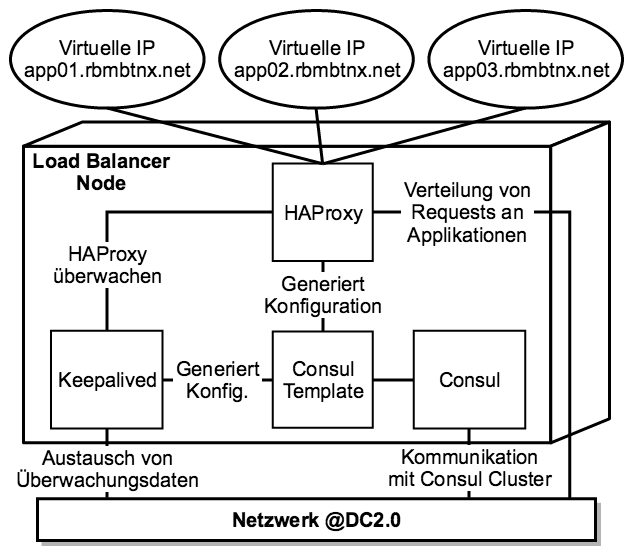
\includegraphics[width=0.7\textwidth]{img/loadbalancer_node.png}
	\caption[Aufbau einer Loadbalancer Node]{Grundsätzlicher Aufbau einer Loadbalancer Node. Alle Komponenten kommen je Node vor und kommunizieren über das Netzwerk.}
	\label{fig:loadbalancer:node}
\end{figure} 

\paragraph{Erfassen der Metriken:}
Die \autoref{tab:metric:loadbalancer} listet die erfassten Metriken für den Aufbau des Loadbalancers. Ein Großteil des Aufwands für die Erstellung des Loadbalancers, war für die Entwicklung des Konzeptes notwendig. Um ein Konstrukt zu ermitteln, das den Anforderungen entspricht, musste zuerst ein Proof of Concept erstellt und getestet werden. Die Erstellung des automatisierten Deployments konnte danach mit wenig Aufwand durchgeführt werden. Hierfür können die Roles für Consul und Supervisor wiederverwendet werden. Dennoch ist durch die Anzahl der Komponenten die Komplexität des Loadbalancers höher als bei Consul, weswegen mehr Aufwand für die Implementierung notwendig war. Der zusätzliche Aufwand je Applikation, für die Integration in den Loadbalancer ist verschwindend gering, da nur der Consul Client installiert werden muss.

\begin{table}[ht]
%\setlength{\arrayrulewidth}{0.3mm}
\setlength{\tabcolsep}{5pt}
\renewcommand{\arraystretch}{1.5}
\centering
\begin{tabular}{|l|l|l|}
\hline
\rowcolor[HTML]{C0C0C0}
\multicolumn{2}{|c|}{\textbf{Metrik}} & \textbf{Menge}					\\ 
\hline
\multirow{3}{*}{Initialer Aufwand}	& Konzept \& Implementation & 230 PS	\\ 
\cline{2-3}
									& wiederverwendete Roles & 2 Stk		\\
\cline{2-3}
									& je Applikation 		& 0 PS 	\\
\hline 
\multirow{2}{*}{Komplexität}			& Anzahl der Komponenten & 5 		\\
\cline{2-3}
									& verteiltes System		& Ja 		\\
\hline
\multirow{3}{*}{Durchlaufzeit} 		& a.) eine Node		& ca. 7 Minuten	\\ 
\cline{2-3} 
									& b.) alle Nodes		& ca. 16 Minuten	\\ 
\cline{2-3}							
									& c.) zusätzliche Node	& ca. 10 Minuten 	\\
\hline
\end{tabular} 
\caption{Erfasste Metriken des Loadbalancers}
\label{tab:metric:loadbalancer}
\end{table}

Der Loadbalancer darf bei einem Update nicht komplett ausgeschaltet werden, ansonsten gibt es Unterbrechungen in der Erreichbarkeit der Applikationen. Daher darf immer nur eine Node nach der anderen aktualisiert werden. Aus diesem Grund ist die Zeit für alle Nodes (b), ähnlich wie bei Consul, die Zeit einer Node (a) mal der Anzahl der Nodes. Allerdings muss der Loadbalancer selten neu provisioniert werden, da die häufige Änderung der Konfiguration von Consul-Template durchgeführt wird.
Das Deployment einer zusätzlichen Node braucht etwas länger als ein erneutes Deployment. Der Grund hierfür ist, wie bei Consul, der Download der Komponenten.

\subsection{Log-Aggregation mit Logstash}
\label{sec:logstash:main}
Im klassischen Betrieb werden Log-Dateien auf den jeweiligen Maschinen gesammelt. Kommt es zu Problemen, können sich die Entwickler auf einer Maschine einloggen und Log-Dateien abrufen. Das setzt voraus, dass entsprechende Zugangsberechtigungen existieren, die für jede neue Maschine eingerichtet werden müssen. Bei DevOps ändert sich allerdings die Infrastruktur häufig. Die Anzahl der Maschinen ist sehr volatil, um beispielsweise auf verschiedene Lastsituationen reagieren zu können. Es erfordert hierbei einen hohen Aufwand, die Zugangsberechtigungen zu verwalten. Um dem Problem entgegenzuwirken, muss ein zentraler Ansatz verfolgt werden. Die Log-Dateien aller Applikationen und Maschinen werden an einer zentralen Stelle gesammelt und können von hieraus von den Entwicklern eingesehen werden. Die Red Bull Media Base setzt im DC2.0 für diese Aufgabe den sogenannten ELK-Stack ein. Dieser besteht aus Logstash\footnote{\url{http://logstash.net/}, Log-Parser auf Basis von Java}, Elasticsearch\footnote{\url{https://www.elastic.co/products/elasticsearch}, NoSQL Datenspeicher} und Kibana\footnote{\url{https://www.elastic.co/products/kibana}, Javascript Applikation zur Datenvisualisierung} \cite{Papaspyrou2014}.

\paragraph{Grundsätzliche Funktionsweise von Logstash:}
Dieses System ermöglicht es, die Log-Nachrichten über sogenannte Log-Shipper, die lokal auf den Maschinen installiert sind, direkt an die zentrale Instanz zu schicken. Somit müssen dem ELK-Stack die Maschinen nicht bekannt sein. Die einzelnen Applikationen schicken automatisch ihre Logs und es ist keine spezielle Konfiguration des ELK-Stacks notwendig. Der ELK-Stack analysiert und indiziert die ankommenden Daten und macht sie für die Benutzer durchsuchbar. Das Schema in Abbildung \ref{fig:logstash:schema} zeigt den grundsätzlichen Aufbau des ELK-Stacks.

\begin{figure}[ht]
	\centering
	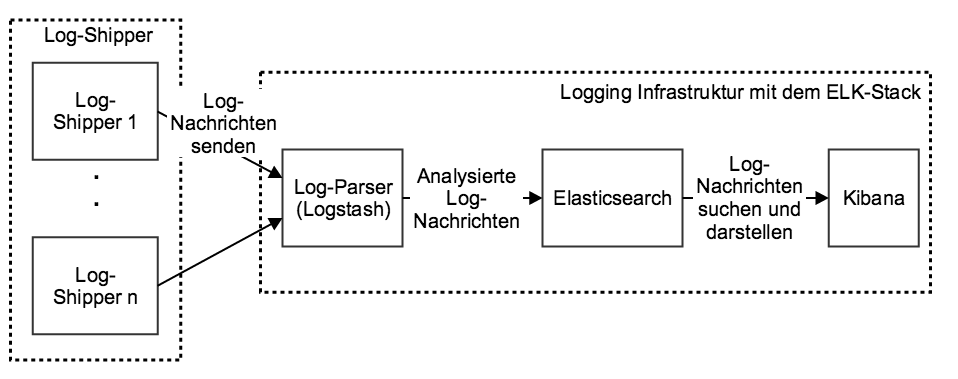
\includegraphics[width=0.97\textwidth]{img/logstash.png}
	\caption[Grundsätzliches Funktionsschema des ELK-Stacks, adaptiert aus \cite{Papaspyrou2014}]{Grundsätzliches Funktionsschema des ELK-Stacks, adaptiert aus \cite{Papaspyrou2014}. Die Pfeilrichtungen geben den Datenfluss zwischen den Komponenten an.}
	\label{fig:logstash:schema}
\end{figure} 

Der ELK-Stack besteht grundsätzlich aus drei Komponenten für die Analyse, Indizierung \& Speicherung sowie Visualisierung der Log-Nachrichten. Die Log-Lieferung kann über diverse Applikationen (siehe Abschnitt \ref{sec:logstash:shipper}) erfolgen und wird üblicherweise nicht zum ELK-Stack gezählt. Sobald ein Client Log-Nachrichten produziert, werden diese vom Log-Shipper an die zentrale Logging Infrastruktur geschickt. Dort werden die Nachrichten von Logstash analysiert und entsprechend aufbereitet. Zu diesem Zeitpunkt ist es möglich, die Log-Nachrichten durch weitere Daten anzureichern oder unnötige Teile zu filtern. Nach erfolgreicher Analyse, werden sie an Elasticsearch weitergeleitet. Elasticsearch indiziert die Daten anhand ihres Erstellungsdatums und speichert sie. Mit Hilfe von Kibana können die Benutzer die Daten aus Elasticsearch abfragen, filtern und entsprechend visualisieren. 

Logstash bietet eine Vielzahl von möglichen Ausgabeformaten\footnote{\url{http://logstash.net/docs/1.4.2/}, Spalte \textit{outputs} bei \textit{plugin documentation}} für Speicher wie Solr, S3 oder Redis an. Es muss nicht Elasticsearch verwendet werden. Allerdings sind die Komponenten im ELK-Stack miteinander bereits erprobt und werden von demselben Unternehmen (Elastic) entwickelt. Die Kompatibilität der einzelnen Komponenten untereinander sollte daher gegeben sein \cite{Papaspyrou2014}.

\paragraph{Aufbau der Logging Infrastruktur:} 
Abbildung \ref{fig:logstash:nodes} zeigt den grundsätzlichen Aufbau der verschiedenen Nodes in der Logging Infrastruktur. Auf der Log-Parser Node (Abbildung \ref{fig:logstash:parsernode}) läuft Logstash als Prozess. Logstash selbst ist eine zustandslose Applikation, in der eine Log-Nachricht immer nur von einem Prozess verarbeitet wird. Es besteht keine Abhängigkeit zu anderen Log-Nachrichten. Daher ist es möglich, mehrere Logstash Instanzen parallel zu betreiben, ohne das Konflikte entstehen. Die Hauptaufgabe der Elasticsearch Nodes (Abbildung \ref{fig:logstash:esnode}) ist die Speicherung und Indizierung der Daten. Elasticsearch ist eine hochperformante NoSQL Datenbank und bietet die Möglichkeit, einen verteilten Cluster zu bilden. Die Daten werden automatisch auf allen operativen Nodes verteilt. Es ist also möglich, mehrere Log-Parser und Elasticsearch Nodes parallel in einem Cluster zu betreiben. Kibana ist eine Javascript Applikation, die auf dem Rechner der Benutzer läuft und muss somit nicht skaliert werden. Da Logstash wie auch Elasticsearch CPU intensive Applikationen sind, werden sie auf unterschiedlichen Nodes getrennt betrieben, um die Last besser zu verteilen.

\begin{figure}[ht]
	\centering
    \begin{subfigure}[b]{0.40\textwidth}
    		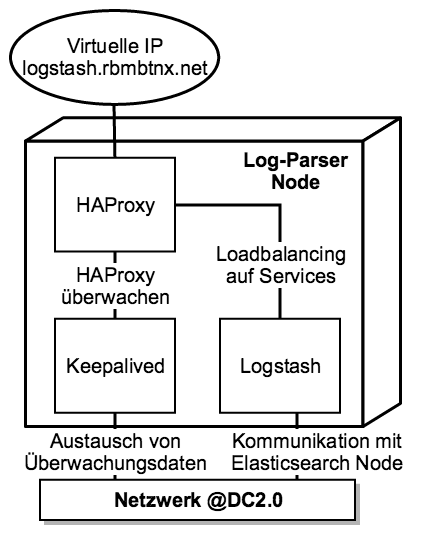
\includegraphics[width=\textwidth]{img/logstash_parser_node.png}
        \caption{Log-Parser Node}
        \label{fig:logstash:parsernode}
    \end{subfigure}
    \begin{subfigure}[b]{0.585\textwidth}
        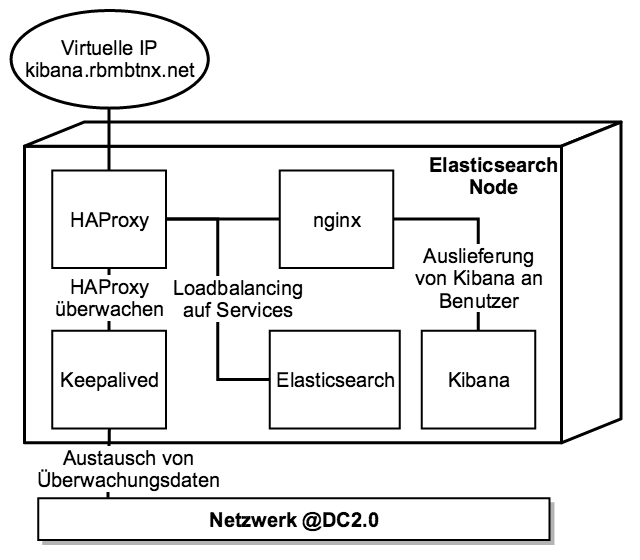
\includegraphics[width=\textwidth]{img/logstash_es_node.png}
        \caption{Elasticsearch Node}
        \label{fig:logstash:esnode}
    \end{subfigure}
    \caption[Aufbau der ELK-Stack Node]{Grundsätzlicher Aufbau der Nodes unseres ELK-Stacks in der Logging Infrastruktur. Alle Komponenten kommen je Typ von Node vor und sie bilden Cluster, um sich über alle Nodes gleichen Typs hinweg zu synchronisieren.}
    \label{fig:logstash:nodes}
\end{figure}

Folgende Aufgaben erfüllen die weiteren Komponenten. Nicht alle Komponenten sind auf beiden Nodetypen installiert, siehe \autoref{fig:logstash:nodes}:
\begin{itemize}
 \item \textbf{Keepalived:} Keepalived übernimmt hierbei dieselbe Aufgabe wie beim Loadbalancer (siehe Abschnitt \ref{sec:loadbalancer}).
 \item \textbf{HAProxy:} Er fungiert als Loadbalancer und verteilt die ankommenden Anfragen auf alle funktionalen Log-Parser/Elasticsearch Nodes im Cluster.
 \item \textbf{nginx\footnote{\url{http://nginx.org/en/}, wird u.a. von Netflix und Wordpress eingesetzt}:} Dies ist ein leichtgewichtiger Webserver, der für die Auslieferung von Kibana an die Benutzer zuständig ist. Außerdem fungiert er als Reverse-Proxy für die Kommunikation von Kibana mit Elasticsearch. Damit werden Daten immer nur von der ursprünglichen Node von Kibana abgefragt und die Last wird verteilt. Außerdem wird damit die CORS\footnote{\url{http://www.w3.org/TR/cors/}, Cross-Origin Resource Sharing} Problematik umgangen.
\end{itemize}

Auf jeder Node des jeweiligen Typs sind alle in Abbildung \ref{fig:logstash:nodes} dargestellten Komponenten installiert. Durch diesen Aufbau ist die Möglichkeit zur horizontalen Skalierung, in allen relevanten Teilen der Logging Infrastruktur, gegeben. Daher ist der ELK-Stack zukunftssicher, im Bezug auf steigende Lastanforderungen und Datenmengen. Außerdem weist dieser Aufbau einen hohen Grad an Ausfallsicherheit auf. Solange jeweils eine Log-Parser und Elasticsearch Node korrekt funktionieren, ist der Service verfügbar. Durch die Replikation der Daten auf alle Elasticsearch Nodes ist es unwahrscheinlich, dass Daten verloren gehen. Es ist nicht anzunehmen, dass der gesamte Cluster innerhalb kurzer Zeit fehlerhaft ist und somit eine Datenrettung nicht mehr möglich ist. Aus diesem Grund kann auf ein Backup verzichtet werden.

\paragraph{Log-Shipper und Konfiguration:}
\label{sec:logstash:shipper}
Für die Log-Lieferung bietet Logstash eine Menge an möglichen Inputs\footnote{\url{http://logstash.net/docs/1.4.2/}, Spalte \textit{inputs} bei \textit{plugin documentation}} an. Im aktuellen Aufbau sind zwei Möglichkeiten der Lieferung umgesetzt, die alle nötigen Anforderungen erfüllen. Diese sind rsyslog\footnote{\url{http://www.rsyslog.com/doc/v8-stable/}, weit verbreitet auf Linux Systemen} und logback\footnote{\url{http://logback.qos.ch/}, Nachfolger von Log4J}. Ersteres ist ein Log-Verarbeitungssystem, das in Linux Distributionen weit verbreitet ist. Mit rsyslog ist es möglich, Log-Dateien auf einer Maschine zu überwachen (ähnlich dem Befehl \textit{tail -f}) und neue Log-Nachrichten an Logstash weiterzuleiten. Der Vorteil hierbei ist, dass an der Applikation keine Änderung notwendig ist, sondern lediglich rsyslog konfiguriert werden muss. Die zweite Möglichkeit, logback, ist ein Logging-Framework für Java Applikationen, das im Umfeld der Red Bull Media Base häufig eingesetzt wird. Logback ermöglicht es, durch Konfiguration sogenannte \textit{Log-Appender} hinzuzufügen. Alle generierten Log-Nachrichten werden an diese weitergeleitet. Auch hier sind keine Änderungen der Applikation notwendig, es muss lediglich ein Log-Appender für Logstash hinzugefügt werden.

Um die Log-Daten entsprechend aufbereiten zu können, werden vier zusätzliche Metadaten definiert, die jede Log-Nachricht enthalten muss. Diese sind:
\begin{itemize}
\item Environment: Info aus welcher Umgebung die Log-Nachricht kommt (Produktion, Pre-Produktion, Staging, Test).
\item Stack: Info zu welchem Applikationsstack die Log-Nachricht gehört.
\item Layer: Info zu welchem Layer eines Applikationsstacks die Log-Nachricht gehört.
\item Datacenter: Info in welchem Rechenzentrum die Applikation steht. Das ist bereits vorbereitend falls zusätzliche Rechenzentren an anderen Standorten aufgebaut werden.
\end{itemize}
Rsyslog sowie logback ermöglichen, die zusätzlichen Metadaten an jede Log-Nachricht hinzuzufügen.

\paragraph{Erfassen der Metriken:}
Die Logging Infrastruktur ist entsprechend der Menge an Komponenten komplex aufzubauen.
\begin{table}[ht]
%\setlength{\arrayrulewidth}{0.3mm}
\setlength{\tabcolsep}{5pt}
\renewcommand{\arraystretch}{1.5}
\centering
\begin{tabular}{|l|l|l|}
\hline
\rowcolor[HTML]{C0C0C0}
\multicolumn{2}{|c|}{\textbf{Metrik}} & \textbf{Menge}					\\ 
\hline
\multirow{3}{*}{Initialer Aufwand}	& Implementation & 120 PS	\\ 
\cline{2-3}
									& wiederverwendete Roles & 3 Stk		\\
\cline{2-3}
									& je Applikation 		& 0 PS 	\\
\hline 
\multirow{3}{*}{Komplexität}		& Anzahl der Komponenten (Log-Parser) & 5 \\
\cline{2-3}
								& Anzahl der Komponenten (Elasticsearch) & 7\\
\cline{2-3}
								& verteiltes System (Beide)		& Ja 	\\
\hline
\multirow{5}{*}{Durchlaufzeit} & a.) eine Node (Log-Parser) & ca. 3 Minuten \\ 
\cline{2-3} 
						& a.) eine Node (Elasticsearch) & ca. 2.5 Minuten \\
\cline{2-3} 

						& b.) alle Nodes					& ca. 19 Minuten	 \\ 
\cline{2-3}							
						& c.) zusätzliche Node (Log-Parser)	& ca. 6 Minuten 		\\
\cline{2-3}
						& c.) zusätzliche Node (Elasticsearch)	& ca. 5 Minuten 	\\
\hline
\end{tabular} 
\caption{Erfasste Metriken der Logging Infrastruktur}
\label{tab:metric:logging}
\end{table}
Allerdings konnten vom Loadbalancer bereits einige Roles für Keepalived, Supervisor und HAProxy wiederverwendet werden, um den Aufwand entsprechend zu reduzieren. Die \autoref{tab:metric:logging} zeigt die konkreten Werte. Im initialen Aufwand inbegriffen, ist die Automatisierung der Installation des Log-Shippers. Dadurch fällt je Applikation nur mehr ein geringer Aufwand an. Um einen unterbrechungsfreien Logging Service zu garantieren und keine Log-Nachrichten zu verlieren, wird bei einem Deployment auf allen Nodes immer eine Node nach der anderen aktualisiert. Aktuell besteht der Logging Cluster aus fünf Nodes. Zwei Log-Parser Nodes und drei Elasticsearch Nodes. Daher ist die Metrik b, wie erwartet ca. fünf mal so lang wie Metrik a. Die Deploymentzeiten einer neuen Node sind etwas länger, was auf den Download der Komponenten zurückzuführen ist. Der längste Download hierbei ist Java, der jedoch bei einem erneuten Deployment entfällt.

\subsection{Monitoring mit Sensu}
\label{sec:sensu:main}
Auch beim Monitoring, muss ein anderer Ansatz als üblich verfolgt werden. In klassischen Umgebungen wird oft Nagios\footnote{\url{http://www.nagios.org/}, weit verbreitetes Monitoring Framework der letzten Jahre} als Monitoring Infrastruktur eingesetzt. Nagios verfolgt einen zentralen Ansatz, bei dem alle Maschinen explizit bei der zentralen Instanz konfiguriert werden müssen. Daher muss die Konfiguration jedes mal angepasst werden, wenn Maschinen erstellt oder entfernt werden. Um dieses Problem zu lösen, muss eine Monitoring Infrastruktur mit dezentralem Ansatz aufgebaut werden. Neue Maschinen sollen sich selbstständig beim Monitoring System anmelden, ohne dieses jedes mal neu konfigurieren zu müssen. Dadurch können Maschinen dynamisch hinzugefügt und entfernt werden, ohne dass manuelle Schritte notwendig sind. Außerdem muss die Monitoring Infrastruktur horizontal skalierbar sein, um steigende Lastanforderungen bewältigen zu können. Die Red Bull Media Base setzt hierfür Sensu\footnote{\url{http://sensuapp.org/}, dezentrale Monitoring Infrastruktur mit Hilfe von Messaging Queues} ein, das die gewünschten Ansätze verfolgt.

\paragraph{Grundsätzliche Funktionsweise von Sensu:}
Sensu ist ein leichtgewichtiges Monitoring Framework, dessen grundsätzlicher Aufbau in Abbildung \ref{fig:sensu_schema} dargestellt ist. Der Sensu Server ist die zentrale Instanz, die alle Monitoring Checks auslöst, auswertet und speichert. Auf den Maschinen läuft jeweils der ressourcensparende Sensu Client, der die konkreten Checks durchführt. Die Kommunikation zwischen Server und Clients erfolgt über eine verteilte Messaging-Queue\footnote{Sensu verwendet hierfür RabbitMQ: \url{https://www.rabbitmq.com/}}, über die Nachrichten dezentral ausgetauscht werden. Der Server sendet über die Queue in regelmäßigen Abständen, Aufforderungen zur Ausführung von Monitoring Checks. Die Clients lauschen auf diese Befehle und führen, sofern für sie relevant, entsprechende Checks aus. Die Last verteilt sich somit, da jeder Client die Checks selbst ausführt und diese nicht vom Server durchgeführt werden. Das Ergebnis der Checks wird über die Messaging-Queue zurück an den Server gesendet, wo diese ausgewertet und am Dashboard dargestellt werden. 

Wird eine zusätzliche Maschine hinzugefügt, so meldet sich diese automatisch beim Server an und es ist keine Änderung der Konfiguration notwendig. Ab diesem Zeitpunkt ist der neue Client dem Server bekannt und dieser muss nur auf die Nachrichten in der Queue achten. Der Server muss somit nicht wissen, wo und wie viele Clients vorhanden sind. Lediglich die Messaging-Queue muss für Beide erreichbar sein. Das Entfernen von Maschinen kann über das Dashboard erfolgen und benötigt ebenso keine Konfigurationsänderung.

\begin{figure}[ht]
	\centering
	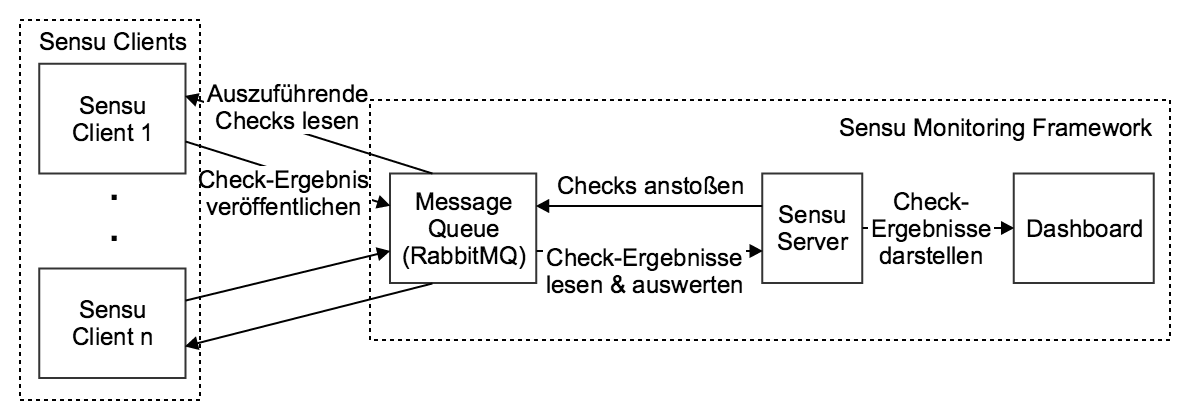
\includegraphics[width=0.999\textwidth]{img/sensu.png}
	\caption[Grundsätzliches Funktionsschema der Sensu Monitoring Infrastruktur]{Grundsätzliches Funktionsschema der Sensu Monitoring Infrastruktur. Die Pfeilrichtungen geben den Datenfluss zwischen den Komponenten an.}
	\label{fig:sensu_schema}
\end{figure}

Das Ergebnis eines Checks kann grundsätzlich zwei Formen annehmen. Herkömmliche Checks überprüfen die korrekte Funktionsweise einer Applikation und liefern grundsätzlich nur \textit{OK} oder \textit{nicht OK} als Ergebnis zurück. Eine spezielle Form der Checks sammelt Metriken (wie beispielsweise aktuelle CUP Last, verbrauchter Speicher, Netzwerkauslastung) über die jeweilige Maschine und wertet diese Anhand von Grenzwerten aus. Wird ein Grenzwert verletzt, so erfolgt eine entsprechende Benachrichtigung. Checks können grundsätzlich in jeglicher Programmiersprache verfasst werden. Die einzigen Voraussetzungen sind, dass die ausführende Maschine eine entsprechende Laufzeitumgebung aufweist und sich der Check an die minimale Spezifikation\footnote{\url{http://sensuapp.org/docs/0.16/checks}, erster Absatz enthält die minimale Spezifikation} hält. Daher können ebenso Nagios Plugins bei Sensu wiederverwendet werden. 

\paragraph{Aufbau der Monitoring Infrastruktur:}
Abbildung \ref{fig:sensu_node} zeigt den grundsätzlichen Aufbau einer Node der Monitoring Infrastruktur. Sensu nutzt ausschließlich Komponenten die clusterfähig sind und sich gegenseitig synchronisieren. Daher ist es möglich, mehrere Nodes aus Abbildung \ref{fig:sensu_node} gleichzeitig nebeneinander zu betreiben und somit ein ausfallsicheres System zu garantieren. Außerdem ist die Möglichkeit zur horizontalen Skalierung bei allen last-intensiven Komponenten gegeben.

Folgende Aufgaben erfüllen die einzelnen Komponenten:
\begin{itemize}
 \item \textbf{Keepalived:} Keepalived übernimmt hierbei dieselbe Aufgabe wie beim Loadbalancer (siehe Abschnitt \ref{sec:loadbalancer}).
 \item \textbf{HAProxy:} HAProxy fungiert als Loadbalancer und verteilt die ankommenden Anfragen auf alle Nodes im Sensu Cluster. Dies sind Zugriffe der Benutzer auf das Dashboard sowie die Kommunikation der Clients mit der Messaging-Queue.
 \item \textbf{Sensu Server/API:} Er verwaltet die Checks und verarbeitet deren Ergebnisse. Alle Instanzen des Servers ermitteln automatisch einen Master um sicherzustellen, dass Aufforderungen für Checks nicht mehrfach gestellt werden. Zusätzlich dazu bietet der Server eine API, über die beispielsweise das Dashboard Daten bezieht.
 \item \textbf{Sensu Dashboard:} Das Dashboard ist die Benutzeroberfläche und zeigt den aktuellen Status aller Clients und ihre letzten Check-Ergebnisse an.
 \item \textbf{RabbitMQ:} Ist eine Messaging-Queue für die Kommunikation zwischen Server und Clients. Alle RabbitMQ Nodes verbinden sich zu einem Cluster und synchronisieren ihre Daten über das Netzwerk hinweg. Es ist somit unerheblich bei welche Node Daten abgefragt werden. Es wird immer das gleiche Ergebnis zurückgeliefert. Der Sensu Server kann also seine lokale RabbitMQ Node nutzen.
 \item \textbf{Redis\footnote{\url{http://redis.io/topics/cluster-tutorial}, Redis Cluster inkl. Replikation der Daten}:} Ist ein Key-Value Store und wird vom Sensu Server genutzt, um Daten zu speichern. Redis persistiert unter anderem die Ergebnisse der Checks über einen gewissen Zeitraum. Folglich ist in Sensu stets eine Historie über die letzten Checks vorhanden. Redis synchronisiert seine Daten ebenfalls über alle Nodes.
 \item \textbf{Redis-Sentinel\footnote{\url{http://redis.io/topics/sentinel}, Redis Node im Sentinel Modus}:} Ist eine Redis Node, die in einem speziellen Modus gestartet wird. Sie ist zuständig für die Überwachung des Redis Clusters und erkennt fehlerhafte Nodes, um diese aus dem Cluster zu entfernen. Alle Redis-Sentinel Nodes synchronisieren sich ebenfalls über das Netzwerk untereinander.
\end{itemize}

\begin{figure}[ht]
	\centering
	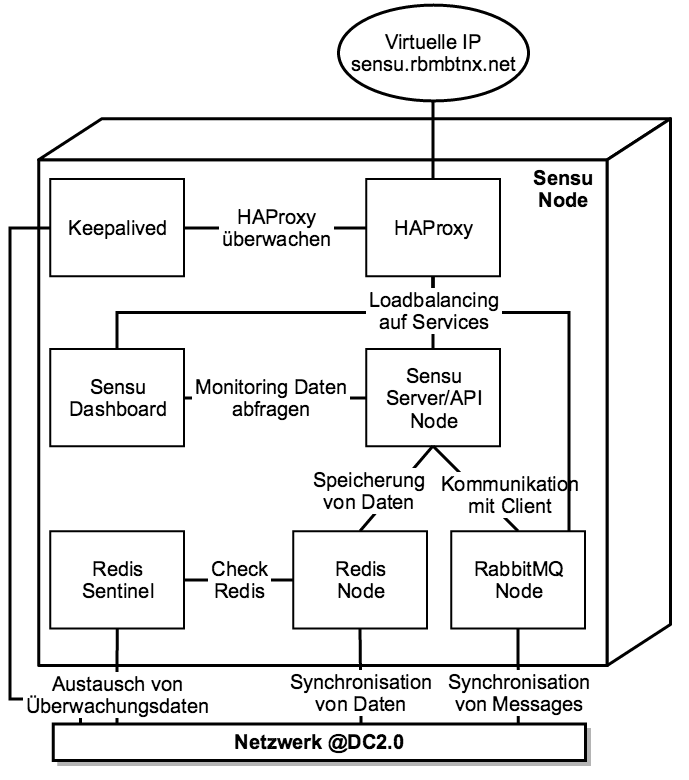
\includegraphics[width=0.7\textwidth]{img/sensu_node.png}
	\caption[Aufbau einer Sensu Node]{Grundsätzlicher Aufbau einer Sensu Node in der Monitoring Infrastruktur. Alle Komponenten sind je Node vorhanden und die meisten Komponenten bilden Cluster, um sich gegenseitig zu synchronisieren.}
	\label{fig:sensu_node}
\end{figure}

Da alle gezeigten Komponenten auf jeder Node installiert sind, müssen nicht mehrere Typen von Nodes unterschieden werden und vereinfacht somit die Verwaltung des Clusters. Dieser Aufbau garantiert ein ausfallsicheres System, da alle Nodes gleichzeitig fehlerhaft sein müssen, um einen kompletten Systemausfall herbeizuführen. Ein weiterer Vorteil von Sensu ist, dass sich die Monitoring Infrastruktur selbst überwachen kann und kein externes System dafür benötigt wird.

Zusätzlich zu den Sensu Nodes existiert eine weitere Maschine, die gesondert behandelt werden muss. Auf dieser Maschine wird Graphite\footnote{\url{http://graphite.wikidot.com/}, leichtgewichtige Datenbank zur Datenaggregierung} und Grafana\footnote{\url{http://docs.grafana.org/}, Javascript Applikation zur Graphenvisualisierung} betrieben. Graphite speichert die Daten der Client-Metriken und aggregiert sie über konfigurierbare Zeiträume. Mittels Grafana können anschließend Graphen erstellt werden, die den zeitlichen Verlauf der Metriken darstellen. Somit ist es möglich, detaillierte Reports über beispielsweise die Last eines Systems zu generieren. Anhand dieser Daten können dadurch potentielle Probleme frühzeitig vorausgesagt werden. Da auf dieser Maschine Daten gespeichert werden, muss sie anders behandelt werden als die Sensu Nodes und darf nicht einfach entfernt und neu aufgebaut werden.

\paragraph{Client Konfiguration:}
\label{sec:sensu_client}
Die Konfiguration der Clients\footnote{\url{http://sensuapp.org/docs/0.16/clients}, Konfiguration des Sensu Clients} enthält Basis-Informationen über den Client selbst und die Zugehörigkeit (\textit{subscriptions}) der Maschine zu einer oder mehreren Applikationsgruppen (siehe Listing \ref{lst:config_da}). Die Gruppen geben an, welche Checks für die jeweilige Maschine relevant sind und ausgeführt werden müssen.

\begin{lstlisting}[style=code,numbers=left,caption={Beispielhafte Client Konfiguration des Delivery Agent},label={lst:config_da}]
{
  "client": {
    "name": "prod-da-app02.rbmbtnx.net",
    "address": "172.20.32.71",
    "subscriptions": ["common","da-application","webserver"],
    "rbmb": {
      "dc": "ffm",
      "env": "prod",
      "stack": "delivery-agent",
      "layer": "application"
    }
  }
}
\end{lstlisting}

Um den Client jederzeit eindeutig im DC2.0 identifizieren und die Daten entsprechend verarbeiten zu können, wurden wie bei Logstash, die vier eigenen Metadaten hinzugefügt. Diese sind in dem Element \textit{rbmb} eingebettet, um keinen Konflikt mit anderen Elementen zu verursachen.

\paragraph{Erfassen der Metriken:}
Für die Monitoring Infrastruktur müssen neun verschiedene Komponenten automatisiert werden. Allerdings konnten die Roles für HAProxy, Supervisor und Keepalived wiederverwendet werden (\autoref{tab:metric:monitoring}). 
\begin{table}[ht]
%\setlength{\arrayrulewidth}{0.3mm}
\setlength{\tabcolsep}{5pt}
\renewcommand{\arraystretch}{1.5}
\centering
\begin{tabular}{|l|l|l|}
\hline
\rowcolor[HTML]{C0C0C0}
\multicolumn{2}{|c|}{\textbf{Metrik}} & \textbf{Menge}					\\ 
\hline
\multirow{3}{*}{Initialer Aufwand}	& Implementation & 150 PS	\\ 
\cline{2-3}
									& wiederverwendete Roles & 3 Stk		\\
\cline{2-3}
									& je Applikation 		& 0 PS 	\\
\hline 
\multirow{2}{*}{Komplexität}			& Anzahl der Komponenten & 9 		\\
\cline{2-3}
									& verteiltes System		& Ja 		\\
\hline
\multirow{3}{*}{Durchlaufzeit} 		& a.) eine Node		& ca. 6 Minuten	\\ 
\cline{2-3} 
									& b.) alle Nodes		& ca. 25 Minuten	\\ 
\cline{2-3}							
									& c.) zusätzliche Node	& ca. 8 Minuten	\\
\hline
\end{tabular} 
\caption{Erfasste Metriken der Monitoring Infrastruktur}
\label{tab:metric:monitoring}
\end{table} 
Man erkennt also bereits die Tendenz, je mehr Applikationen automatisiert wurden, desto mehr Roles sind wiederverwendbar. Der initiale Aufwand der Implementierung ist dennoch hoch, da die Monitoring Infrastruktur viele Komponenten verwendet, die bisher nicht eingesetzt wurden. Wie bei Logstash ist auch hier die Installation des Clients mit eingerechnet. Der Aufwand pro Applikation ist daher verschwindend gering. Es müssen lediglich Monitoring Checks erstellt werden, sofern die vorhandenen Checks nicht ausreichend sind. Dieser Aufwand reduziert sich daher bei steigender Anzahl der Applikationen erheblich. Um einen unterbrechungsfreien Monitoring Service zu garantieren, wird bei einem Deployment auf allen Nodes immer nur eine Node zur gleichen Zeit aktualisiert. Aktuell besteht der Sensu Cluster aus vier Nodes: drei Sensu Nodes und einer Node mit Graphite. Daher ist die Metrik b (Deployment auf allen Nodes) auch wie erwartet etwa vier mal so lang wie Metrik a (Deployment auf einer Node). Das Deployment einer zusätzlichen Node ist im Vergleich zu Logstash weniger stark angestiegen. Ein Grund hierfür ist, dass die Komponenten von Sensu geringere Dateigrößen aufweisen und somit der Download schneller abgeschlossen ist. Es ist daher die Tendenz erkennbar, dass je größer die Dateien sind die benötigt werden, desto höher ist der Anstieg der Zeit für ein neues Deployment im Vergleich zu einem Re-Deployment.

\subsection{Zusammenfassung der Basisinfrastruktur}
\label{sec:zusammenfassung:basisinfrastruktur}
Zusammenfassend betrachtet fallen für den Aufbau der Basisinfrastruktur Aufwände von ca. 628 Personenstunden an. Sofern von den Systemen und Konzepten aus Abschnitt \ref{sec:systemeundkonzepte} noch nichts bestehendes vorhanden ist, fallen dafür noch einmal zusätzlich 210 Personenstunden an. Insgesamt ergibt sich somit ein Aufwand von 838 Personenstunden, der aufgeteilt auf die drei Personen des Projektteams, eine minimale Durchlaufzeit von knapp sieben Wochen ergibt. Der Aufbau der Basisinfrastuktur kann daher in etwa zwei Monaten abgeschlossen werden und benötigt nur ein Drittel der verfügbaren Zeit. Betrachtet man die Aufwände genauer, ist zu erkennen, dass es sich fast nur um einmalige Aufwände handelt. Die Entwicklung der Konzepte, sowie der Aufbau der Applikationen muss nur einmalig durchgeführt werden. Lediglich bei der Erstellung der virtuellen Maschine und der Integration in den Consul Cluster ist ein Aufwand je Applikation erforderlich. Sofern komplett neue Komponenten betrieben werden, müssen entsprechende Monitoring Checks erstellt werden. Steigt die Anzahl der Komponenten, steigt auch die Anzahl der vorhandenen Checks. Diese können somit wiederverwendet werden, was den wiederkehrenden Aufwand gering hält.

\section{Implementierung der DevOps Konzepte}
Die nachfolgenden Abschnitte befassen sich mit dem zweiten Teil der Fallstudie. Es werden insgesamt vier Applikationen beschrieben, bei denen die Konzepte von DevOps eingeführt wurden. Je Applikation wird zuerst ihr aktueller Aufgabenbereich  beschrieben. Anschließend wird auf den Aufbau der Applikation genauer eingegangen, um einen Überblick über dessen Komplexität zu geben. Als Nächstes wird die Implementierung beschrieben. Hierbei wird im Besonderen auf neue Bestandteile eingegangen und welche Teile von anderen Applikationen wiederverwendet wurden. Abschließend werden die Metriken erfasst und erklärt.

\subsection{Applikation - Delivery Agent}
\label{sec:deliveryagent}
Ein wiederkehrender Anwendungsfall bei vielen Applikationen, ist die Auslieferung von Multi-Media-Ressourcen an die Benutzer. Vorschaubilder oder Proxies für Videodateien, wie im Outlet\footnote{\url{www.redbullcontentpool.com}} der Red Bull Media Base, sind Ressourcen die häufig benötigt werden. Damit nicht jede Applikation diese Funktionalität bereitstellen muss, wurde sie in eine eigene Applikation namens Delivery Agent ausgegliedert. Dieser ist dafür zuständig, Ressourcen durch unterschiedliche Abgriffsmethoden (Progressive Download, Streaming, etc.) bereitzustellen. Applikationen die Ressourcen benötigen, können diese über Links einbinden und somit vom Delivery Agent ausliefern lassen. Durch den begrenzten Aufgabenbereich des Delivery Agents, ist dieser Teil der weniger komplexen Applikationen, die im Zuge der Fallstudie betrachtet werden. Allerdings gelten für ihn spezielle Anforderungen an den Betrieb. Da er einen der häufigsten Anwendungsfälle bedient, ist die Last auf diesem System entsprechend hoch. Der Delivery Agent muss mit dieser hohen Last umgehen können. Außerdem stellt er eine grundlegende Funktionalität bereit und muss deswegen entsprechend ausfallsicher sein. Ansonsten wäre die Funktionalität der abhängigen Applikationen beeinträchtigt.

\paragraph{Aufbau der Applikation:}
Um die, im vorherigen Absatz beschriebenen, Anforderungen erfüllen zu können, muss der Delivery Agent als verteiltes System aufgebaut sein. Der Delivery Agent ist eine zustandslose Applikation und erleichtert somit die Verteilung des Systems, da keine Daten zwischen den unterschiedlichen Nodes synchronisiert werden müssen. Die \autoref{fig:da_node} zeigt den grundsätzlichen Aufbau einer Delivery Agent Node. Durch die zustandslose Arbeitsweise der Komponenten, können beliebig viele Nodes parallel betrieben werden und es ist keine Clusterbildung notwendig. Durch diese Möglichkeit zur horizontalen Skalierung, lassen sich zukunftssicher, steigende Lastanforderungen bewältigen. Folgende Aufgaben führen die einzelnen Komponenten aus:

\begin{itemize}
	\item \textbf{Delivery Agent:} Ist eine Spring-Boot-Applikation\footnote{\url{http://projects.spring.io/spring-boot/}, Framework für Standalone Applikation mit Java} die für die Verwaltung und Auslieferung der Ressourcen zuständig ist. Sie fordert die Lage der Ressourcen von einer zentralen Instanz an und stellt diese anschließend bereit.
	\item \textbf{nginx:} Der nginx Webserver übernimmt das Caching von häufig angefragten Ressourcen, um diese schneller ausliefern zu können. Ist eine Ressource nicht im Cache vorhanden, so wird die Anfrage an die Delivery Agent Komponente weitergeleitet.
	\item \textbf{Consul:} Um Ausfallsicherheit und optimale Lastverteilung zu erreichen, ist der Delivery Agent an den globalen Loadbalancer des DC2.0 angeschlossen. Wie in Abschnitt \ref{sec:loadbalancer} beschrieben, ist hierfür der Consul Client auf der Node notwendig.
	\item \textbf{Sensu-Client:} Damit die Node entsprechend vom Monitoring System überwacht wird, ist der Sensu-Client erforderlich. Dieser überwacht die Komponenten und führt Checks durch, ob diese noch korrekt funktionieren.
	\item \textbf{Log-Shipper:} Die Log-Dateien der einzelnen Komponenten werden an das zentrale Logging System aus Abschnitt \ref{sec:logstash:main} geschickt. Diese Aufgabe wird vom Log-Shipper (in diesem Fall logback) übernommen.
\end{itemize}

\begin{figure}[ht]
	\centering
	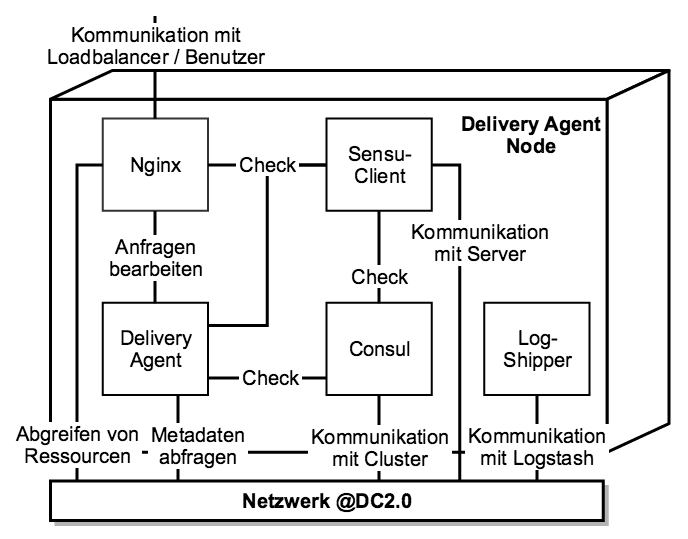
\includegraphics[width=0.7\textwidth]{img/deliveryagent_node.png}
	\caption[Aufbau einer Delivery Agent Node]{Grundsätzlicher Aufbau einer Delivery Agent Node. Alle Komponenten kommen pro Node vor. Die Nodes sind unabhängig voneinander und teilen keine Daten.}
	\label{fig:da_node}
\end{figure} 

Zusätzlich zu den oben beschriebenen Komponenten, sind auch noch die Java Runtime Umgebung sowie Supervisor für die Verwaltung der Komponenten installiert.

\paragraph{Automatisierung des Deployments:}
Da der Delivery Agent den globalen Loadbalancer nutzt, muss kein dedizierter Loadbalancer aufgebaut werden. Durch die Implementierung der Basisinfrastruktur sind bereits Roles für die Komponenten Java, nginx, Supervisor, Sensu-Client, Log-Shipper und Consul vorhanden. Hierbei ergibt sich bereits ein hohes Maß an Wiederverwendbarkeit. Bei der Automatisierung des Deployments reduziert sich deswegen der Aufwand auf ein Minimum, da nur die Installation der Delivery Agent Komponente und die Konfiguration zweier Komponenten betrachtet werden muss. Die Roles für den nginx und Supervisor sind sehr allgemein gehalten, um sie wiederverwenden zu können. Aus diesem Grund müssen beide für den konkreten Anwendungsfall des Delivery Agent noch speziell konfiguriert werden.

Zusätzlich zur Automatisierung des Deployments, müssen für den Delivery Agent noch Formation Roles (Abschnitt \ref{sec:formation}) für die virtuellen Maschinen, sowie entsprechende Build und Deploymentpläne in Bamboo (Abschnitt \ref{sec:pipeline}) angelegt werden. Nachdem diese Tätigkeiten beendet wurden, konnte der Delivery Agent vollständig automatisiert deployed werden. Es sind keine manuellen Schritte mehr notwendig.

\paragraph{Erfassen der Metriken:}
Der initiale Aufwand der Implementierung für den Delivery Agent fällt sehr gering aus, da nur eine einzige weitere Komponente automatisiert werden musste. Auch die Verteilungsaspekte des Delivery Agent haben den Aufwand nicht erhöht. Der Delivery Agent wurde bereits im DC1.0 betrieben. Aus diesem Grund wird ein Vergleich der Deploymentzeiten vor und nach der Automatisierung durchgeführt. 
\begin{table}[ht]
%\setlength{\arrayrulewidth}{0.3mm}
\setlength{\tabcolsep}{5pt}
\renewcommand{\arraystretch}{1.5}
\centering
\begin{tabular}{|l|l|l|}
\hline
\rowcolor[HTML]{C0C0C0}
\multicolumn{2}{|c|}{\textbf{Metrik}} & \textbf{Menge}					\\ 
\hline
\multirow{2}{*}{Initialer Aufwand}	& Implementation & 80 PS	\\ 
\cline{2-3}
									& wiederverwendete Roles & 6		\\
\hline 
\multirow{2}{*}{Komplexität}			& Anzahl der Komponenten & 7 		\\
\cline{2-3}
									& verteiltes System		& Ja 		\\
\hline
\multirow{3}{*}{Durchlaufzeit: Vorher} & a.) eine Node		& ca. 20 Minuten	\\ 
\cline{2-3} 
									& b.) alle Nodes		& ca. 40 Minuten	\\ 
\cline{2-3}							
									& c.) zusätzliche Node	& ca. 90 Minuten \\
\hline
\multirow{3}{*}{Durchlaufzeit: Nacher} & a.) eine Node	& ca. 7 Minuten	\\ 
\cline{2-3} 
									& b.) alle Nodes		& ca. 15 Minuten	\\
\cline{2-3}
									& c.) zusätzliche Node	& ca. 10 Minuten\\
\hline
\end{tabular} 
\caption{Erfasste Metriken des Delivery Agents}
\label{tab:metric:deliveryagent}
\end{table}
Wie in \autoref{tab:metric:deliveryagent} ersichtlich, betrug die Zeit vor der Automatisierung, ca. 20 Minuten für ein Deployment und ca. 1.5 Stunden für das Deployment einer zusätzlichen Node. Nach der Automatisierung benötigt ein Deployment ca. 7 Minuten und das Deployment einer zusätzlichen Node ca. 10 Minuten. Die Provisionierung einer Node ist daher fast dreimal bzw. neunmal so schnell als zuvor. Außerdem waren vor der Automatisierung die Mitarbeiter die komplette Zeit beschäftigt und somit nicht verfügbar. Nach der Automatisierung ist auch während eines Deployments keine menschliche Ressource belegt und kann somit anderen Tätigkeiten nachgehen. Der Zeitgewinn bei der Verfügbarkeit der Mitarbeiter ist somit enorm.

Im aktuellen Setup sind zwei Delivery Agent Nodes vorhanden. Im manuellen Fall muss eine Node nach der anderen aktualisiert werden. Die Zeit für die Belegung der Mitarbeiter multipliziert sich also mit der Anzahl der Nodes. Im automatisierten Fall können alle Nodes, bis auf Eine\footnote{Um einen unterbrechungsfreien Service zu garantieren.}, zur gleichen Zeit aktualisiert werden. Somit beträgt die insgesamt benötigte Zeit, nur die doppelte Zeit einer Node. Der Zeitgewinn beträgt hierbei bereits 26 Minuten (40 gegenüber 14 Minuten). Der Zeitgewinn bei einem Deployment ist daher umso größer, je mehr Nodes vorhanden sind. Es können zwar mehrere Mitarbeiter gleichzeitig arbeiten, dies belegt aber auch entsprechend viele Ressourcen und hat höhere Kosten zur Folge. 


\subsection{Applikation - OAuth2 Server (OIDC)}
\label{sec:oidc}
Nahezu jedes Unternehmen benötigt Applikationen für die Authentifizierung und Autorisierung von Benutzern. Häufig wird dafür ein LDAP System, wie zum Beispiel OpenLDAP, eingesetzt. Nutzen nur interne Applikationen diese Informationen, sind die Sicherheitsanforderungen an diese Systeme gering. Sobald auch andere, externe Applikationen diese Infrastruktur nutzen möchten, müssen umfassende Sicherheitsmaßnahmen ergriffen werden. Bei LDAP besteht allerdings das Problem, dass die Applikation beim Login die Passwörter der Benutzer im Klartext vernehmen und diese unter bösem Vorwand speichern kann. Um dieses Problem zu umgehen, gibt es sichere Alternativen wie OAuth2\footnote{\url{http://tools.ietf.org/html/rfc6749}, Standard für sichere Authentifizierung mittels Tokens.}. Dieser Standard beschreibt eine Möglichkeit, wie sich Benutzer an einem sicheren, zentralen Server anmelden können und dann mittels Tokens bei der jeweiligen Applikation authentifiziert und autorisiert werden. Die nutzende Applikation erhält somit nicht mehr das Passwort im Klartext.

Die Red Bull Media Base betreibt bisher ein eigenes LDAP, das auch von Applikationen anderer Abteilungen genutzt wird. Aus den oben genannten Gründen hat man sich entschieden, das LDAP durch OpenID Connect (OIDC)\footnote{\url{http://openid.net/specs/openid-connect-core-1_0.html}, Spezifikation von OIDC} abzulösen. OpenID Connect ist ein Standard, der auf OAuth2 basiert und diesen um SingleSignOn Funktionalitäten erweitert. Da dieser Service einen zentralen Bestandteil darstellt und viele Applikationen davon abhängen, muss hier besonders auf Ausfallsicherheit geachtet werden.

\paragraph{Aufbau der Applikation:}
Da der OIDC Server im AUTH Subnetz stationiert ist, muss neben dem eigentlichen Service auch ein eigener Loadbalancer und Consul Cluster aufgebaut werden. Die Installation dieser beiden Applikationen ist bereits automatisiert und somit fällt nur minimaler Mehraufwand an. Damit Ausfallsicherheit des Service erreicht wird, muss der OIDC Server als Cluster mit mehreren Nodes betrieben werden. Da jede Node selbst Daten erzeugt, müssen diese synchronisiert werden. Folgende, in \autoref{fig:oidc} dargestellten Komponenten kommen je Node vor:

\begin{itemize}
	\item \textbf{Connect2ID\footnote{\url{http://connect2id.com/products/server}, kommerzielles Produkt zur Nutzung von OIDC}:} Der Connect2ID Server implementiert den OIDC Standard und stellt die grundlegenden Funktionalitäten für die Nutzung von OIDC bereit. Er ist die Hauptkomponente der Node, die von anderen Komponenten genutzt wird.
	\item \textbf{OpenLDAP\footnote{\url{http://www.openldap.org/project/}, Open Source LDAP Implementierung}:} Ist die Datenbank der Node und enthält Informationen über die Benutzer, die vom Connect2ID Server abgerufen werden, um die Berechtigungen der Benutzer zu ermitteln. Außerdem wird die Gültigkeit von Tokens gespeichert.
	\item \textbf{OIDC Login Service:} Diese Komponente ist eine eigens entwickelte Applikation und bietet die Login Maske für die Benutzer, um sich beim OIDC Server zu authentifizieren. Applikationen leiten die Benutzer hierauf weiter, um die Authentifizierung durchzuführen und anschließend Tokens zu erhalten.
	\item \textbf{Password Grant Handler:} Diese Komponente implementiert den Password Grant Flow des OAuth2 Standards. Dieser Grant ist im OIDC Standard nicht enthalten, da hierbei dasselbe Problem mit den Passwörtern im Klartext besteht. Um bestehende Anbindungen von Applikationen noch zu unterstützen, wird dieser Grant temporär angeboten.
	\item \textbf{Consul:} Für den eigenen Consul Cluster im AUTH Subnetz ist ebenfalls der Client notwendig. Er wird ebenso für die Integration in den Loadbalancer genutzt.
	\item \textbf{Sensu-Client / Log-Shipper:} Selbe Funktion wie beim Delivery Agent aus Abschnitt \ref{sec:deliveryagent}.
\end{itemize}

\begin{figure}[ht]
	\centering
	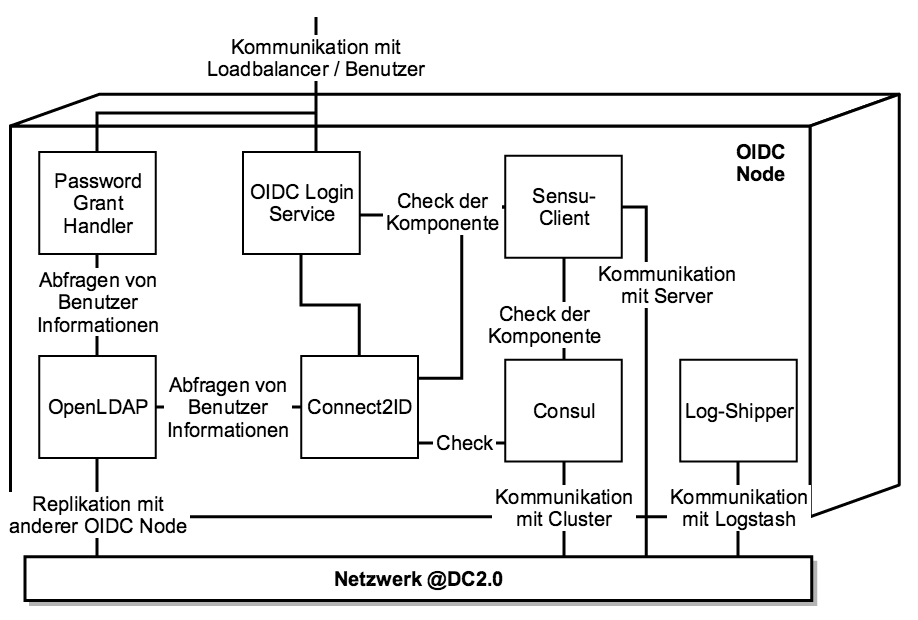
\includegraphics[width=0.7\textwidth]{img/oidc_node.png}
	\caption[Aufbau einer OIDC Node]{Grundsätzlicher Aufbau einer OIDC Node. Alle Komponenten kommen pro Node vor. Alle Nodes verbinden sich zu einem Cluster, um Daten im OpenLDAP zu synchronisieren.}
	\label{fig:oidc}
\end{figure} 

Zusätzlich zu den oben beschriebenen Komponenten sind auch noch die Java Runtime Umgebung, sowie Supervisor für die Verwaltung der Komponenten installiert. Der Connect2ID Server, OIDC Login Service und Password Grant Handler nutzen außerdem einen Tomact Webserver. Dieser wird von den drei Applikationen geteilt.

Bei der Clusterbildung stellte die Synchronisation der Daten das schwerwiegendste Problem dar. Da OpenLDAP als Datenbank genutzt wird, müssen dessen Daten synchronisiert werden. Allerdings ist OpenLDAP nicht für einen verteilten Betrieb ausgelegt. Es bietet zwar klassische Master-Slave Szenarien an, wobei diese hier nicht praktikabel sind, da Daten auf jeder Node des OIDC Cluster geschrieben werden. Bei Master-Slave Szenarien sind Schreiboperationen nur auf einer Node erlaubt. OpenLDAP bietet nur eine Konfiguration, bei der auf mehreren Nodes gleichzeitig geschrieben werden kann, den sogenannten Mirror-Mode. Dieser Modus unterstützt aber maximal zwei Nodes, weswegen der OIDC Cluster auf diese Zahl beschränkt ist. Dies erfüllt die grundlegende Anforderung der Ausfallsicherheit, ist aber kein optimales Setup, da nicht weiter skaliert werden kann. Auf Grund fehlender Alternativen wurde dieses Setup aber umgesetzt.

\paragraph{Automatisierung des Deployments:}
Durch die hohe Anzahl an Komponenten und die Einschränkungen von OpenLDAP, ist der OIDC Server die komplexeste Applikation, die in der Fallstudie betrachtet wird. Auf Grund bisheriger Arbeiten sind bereits Roles für die Komponenten Java, Supervisor, Consul, Sensu-Client und den Log-Shipper vorhanden. Bei der Implementierung müssen noch fünf weitere Komponenten betrachtet werden. Der Tomcat, die beiden selbst entwickelten Applikationen, sowie der Connect2ID Server stellen hierbei kein Problem dar, da sie mit aktuellen Technologien entwickelt wurden. Deren Automatisierung konnte deshalb in angemessener Zeit abgeschlossen werden. Ein Problem stellt die Automatisierung von OpenLDAP dar. OpenLDAP wurde 1998 gestartet und damals wurden noch keine Konzepte für Automatisierung und für einen verteilten Betrieb berücksichtigt. Auch neuere Versionen (2.4) unterstützen diese Konzepte noch nicht vollständig. Vor allem die Konfiguration der OpenLDAP Instanzen ist problematisch. Ein Großteil der Konfiguration ist in der Datenbank gespeichert. Es unterstützt jedoch keine idempotenten Prozesse, weswegen bereits vorhandene Konfigurationen Fehler erzeugen, sofern sie erneut importiert werden. Dies muss bei der Automatisierung speziell berücksichtigt werden. Manche Teile der Konfiguration müssen außerdem auf beiden Nodes importiert werden, andere Teile der Konfiguration nur auf einer Node, da diese anschließend auf die weitere Node synchronisiert wird. Weiters dürfen nicht beide Nodes gleichzeitig aktualisiert werden, da andernfalls die Replikation fehlerhaft sein kann. Deswegen ist es vergleichsweise Komplex, die Automatisierung von OpenLDAP umzusetzen.

Wie für alle Applikationen, müssen zusätzlich noch Formation Roles und Deploymentpläne angelegt werden. Dies betrifft hier auch den Consul Cluster und den Loadbalancer, die extra für das AUTH Subnetz aufgebaut werden. Nach Beendigung dieser Arbeit konnte der OIDC Cluster vollständig automatisiert deployed werden.

\paragraph{Erfassen der Metriken:}
OIDC wurde bisher im DC1.0 nicht eingesetzt, weswegen ein Vergleich der Zeiten nicht möglich ist. Die Anzahl der Komponenten und Roles beziehen sich hierbei rein auf den OIDC Server. Der Consul Cluster und der Loadbalancer werden hierbei nicht berücksichtigt. Deren Metriken können aus dem jeweiligen Abschnitt (\ref{sec:consul} und \ref{sec:loadbalancer}) entnommen werden.
\begin{table}[ht]
%\setlength{\arrayrulewidth}{0.3mm}
\setlength{\tabcolsep}{5pt}
\renewcommand{\arraystretch}{1.5}
\centering
\begin{tabular}{|l|l|l|}
\hline
\rowcolor[HTML]{C0C0C0}
\multicolumn{2}{|c|}{\textbf{Metrik}} & \textbf{Menge}					\\ 
\hline
\multirow{2}{*}{Initialer Aufwand}	& Implementation & 300 PS	\\ 
\cline{2-3}
									& wiederverwendete Roles & 4		\\
\hline 
\multirow{2}{*}{Komplexität}			& Anzahl der Komponenten & 10		\\
\cline{2-3}
									& verteiltes System		& Ja 		\\
\hline
\multirow{3}{*}{Durchlaufzeit} & a.) eine Node		& ca. 12 Minuten	\\ 
\cline{2-3} 
									& b.) alle Nodes		& ca. 28 Minuten	\\ 
\cline{2-3}							
									& c.) zusätzliche Node	& ca. 20 Minuten \\
\hline
\end{tabular} 
\caption{Erfasste Metriken des OIDC Servers}
\label{tab:metric:oidc}
\end{table}
Durch die hohe Anzahl an Komponenten, für die keine Automatisierung vorhanden war, fällt der Aufwand entsprechend höher aus. Es ist bereits die Tendenz erkennbar, dass je homogener die Applikationslandschaft eines Unternehmens ist, desto geringer ist der Aufwand für weitere Applikationen. Ein weiterer Grund für den hohen Aufwand bestand darin, dass im Projektteam bisher wenig Erfahrung mit OpenLDAP vorhanden war. Im aktuellen Fall ist es das erste Mal, dass die Verteilung der Applikation direkte Auswirkungen auf den Aufwand hat. Der Grund hierfür ist OpenLDAP, da es diese Konzepte kaum unterstützt.

Da für einen unterbrechungsfreien Service ohnehin nur eine Node zur gleichen Zeit aktualisiert werden kann, ist diese Einschränkung von OpenLDAP vernachlässigbar. Ein Deployment des gesamten Clusters benötigt ca. 28 Minuten. Auffallend ist der große Unterschied zwischen einem Deployment (a) und dem Deployment einer zusätzlichen Node (c). Dies ist einerseits zurückzuführen auf den Import des Schemas in OpenLDAP, der hier durchgeführt wird und andererseits dem Download der vielen Komponenten.

\subsection{Applikation - Content Processing Agent (CPAS)}
\label{sec:cpas}
Zusätzlich zur Zentrale des Red Bull Media House in Salzburg, gibt es Außenstellen die weltweit verteilt sind. Diese befinden sich in London, Los Angeles, Sydney, Sao Paulo, Frankfurt und Wien. Häufig müssen Multimedia Dateien zwischen diesen Standorten ausgetauscht werden. Das Transcodieren der Dateien ist ebenfalls eine häufig anfallende Aufgabe. Um diese Prozesse zu vereinheitlichen und auch direkt in einer Außenstelle durchführen zu können, wurde der Content Processing Agent (kurz CPAS) entwickelt. Der CPAS ist eine Applikation, die alle nötigen Werkzeuge beinhaltet, um Multimedia Dateien zu verarbeiten. Er steht in Verbindung mit der zentralen Asset-Management-Plattform und erhält von dort Aufgaben, die er durchführt. So können in einer Außenstelle ebenfalls Transcodings bearbeitet werden, und die Dateien müssen nicht zuerst zum zentralen Trancodingcluster transferiert werden. Diese Vorgehensweise spart erheblich Zeit. Außerdem können die CPAS in unterschiedlichen Standorten, Dateien über ein optimiertes Protokoll transferieren. Dieses Protokoll ermöglicht eine bessere Auslastung der verfügbaren Bandbreite. 

Der CPAS kann als zustandslose Applikation betrachtet werden, da er keine Daten mit anderen CPAS Instanzen teilt. Er speichert immer nur die Daten, die für die Verarbeitung seiner aktuellen Aufgaben nötig sind. Die Verwaltung der Aufgaben aller CPAS Instanzen übernimmt die zentrale Asset-Management-Plattform. Ein CPAS kennt eine andere Instanz nur dann, wenn er einen Transfer dorthin durchführt. Es ist also möglich mehrere CPAS Instanzen nebeneinander zu betreiben, ohne das diese miteinender synchronisiert werden müssen.

\paragraph{Aufbau der Applikation:}
Die zentrale Plattform kennt alle CPAS Instanzen und verteilt die Aufgaben gleichmäßig. Daher muss beim CPAS nicht auf Ausfallsicherheit geachtet werden und es ist kein Loadbalancing notwendig. Auch wird in den Außenstellen meist nur eine CPAS Instanz betrieben, da diese Kapazitäten ausreichen. Einzig in den Rechenzentren in Salzburg und Frankfurt werden mehrere CPAS Instanzen bereitgestellt, um höhere Kapazitäten beim Transcoding zur Verfügung zu haben. Nahezu alle Komponenten am CPAS sind für die Verarbeitung von Multimedia Dateien ausgelegt. Die einzelnen Komponenten, wie in \autoref{fig:cpas} dargestellt, sind:

\begin{itemize}
	\item \textbf{CPAS Applikation:} Diese Komponente wurde selbst entwickelt und nutzt die anderen Komponenten zur Verarbeitung von Dateien. Sie kommuniziert mit der zentralen Plattform und erhält von dort ihre Aufgaben. Diese werden an die zuständigen Komponenten weiter verteilt. Gleichzeitig regelt diese Komponente den Zugriff auf den Speicher, um Dateien und berechnete Derivate zu lesen bzw. zu schreiben.
	\item \textbf{Transcoder (ffmpeg)\footnote{\url{https://www.ffmpeg.org/about.html}, weit verbreiteter Open Source Transcoder}:} Der CPAS setzt ffmpeg als Transcoder ein. Über ffmpeg wird die Berechnung von statischen Derivaten durchgeführt, wie beispielsweise Proxies für die Voransicht eines Videos oder die Berechnung eines gewünschten Bestellformats für Kunden.
	\item \textbf{MP4Box\footnote{\url{http://gpac.wp.mines-telecom.fr/mp4box/}, Open Source Multimedia Paketierungssystem}:} Wird für die Aufbereitung von Videos genutzt, um diese per Stream (HTTP Adaptive Streaming) zur Verfügung stellen zu können.
	\item \textbf{Media Processing Service (MPS)\footnote{\url{http://www.lesspain-software.com/products/}, Transcoding Service auf Java Basis}:} Ist ein eigener Service, der auf dem CPAS läuft, um aus Video-Dateien Subclips zu erzeugen. Dieser Vorgang spart in der Post-Produktion Zeit, da dort oftmals nur kleine Teile eines Videos benötigt werden. 
	\item \textbf{UDT Agent:} Ist eine eigens entwickelte Applikation, die für Transfers zwischen den CPAS Instanzen zuständig ist. Sofern an der Quelle und am Ziel ein UDT Agent vorhanden ist, können die Dateien mit dem UDT Protokoll\footnote{\url{http://udt.sourceforge.net/}, Protokoll auf UDP Basis mit eigener Transfersicherheit} optimiert transferiert werden.
	\item \textbf{Sensu-Client / Log-Shipper:} Selbe Funktion wie beim Delivery Agent aus Abschnitt \ref{sec:deliveryagent}.
\end{itemize}

\begin{figure}[ht]
	\centering
	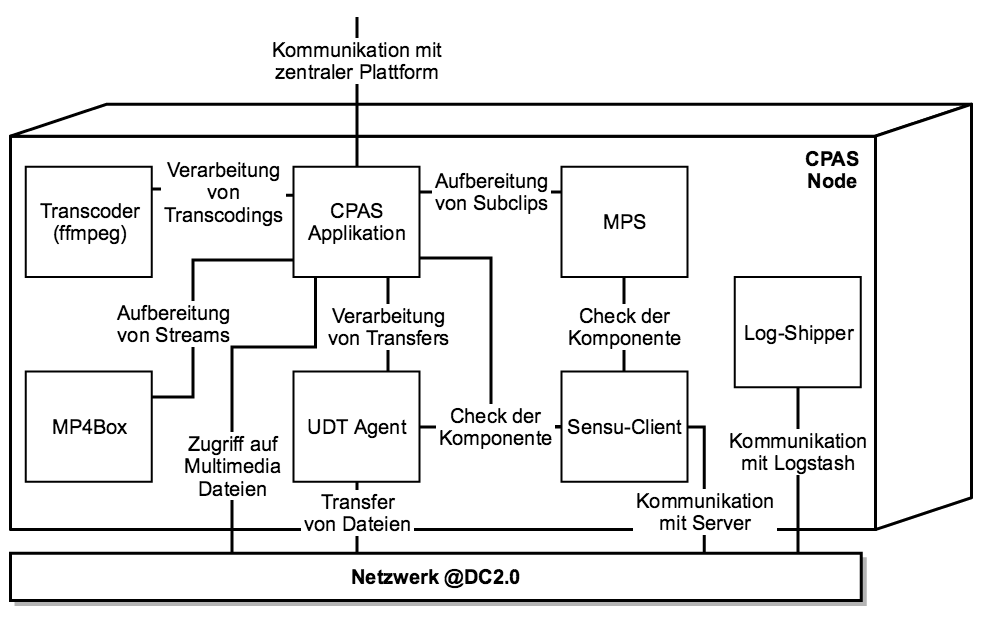
\includegraphics[width=0.7\textwidth]{img/cpas_node.png}
	\caption[Aufbau einer CPAS Node]{Grundsätzlicher Aufbau einer CPAS Node. Alle Komponenten kommen pro Node vor und agieren unabhängig von anderen CPAS Instanzen.}
	\label{fig:cpas}
\end{figure} 

Zusätzlich zu den oben beschriebenen Komponenten, sind noch die Java Runtime Umgebung in zweifacher Ausführung (Version 7 für CPAS und Version 8 für MPS), sowie Supervisor für die Verwaltung der Komponenten installiert. Der UDT Agent benötigt außerdem einen Tomact Webserver als Laufzeitumgebung.

\paragraph{Automatisierung des Deployments:}
Bei der Automatisierung des Deployments muss beim CPAS, vor allem auf die Unterschiede zwischen den einzelnen Standorten geachtet werden. So müssen an jedem Standort andere Speichersysteme eingebunden werden. Dies wurde hauptsächlich über Ansible Variablen abgebildet, die abhängig vom jeweiligen Standort des CPAS geladen werden. So kann derselbe Code für das Mounten der Speichersysteme verwendet werden. Ansonsten gibt es keine Unterschiede zwischen den Standorten, die beim Deployment speziell berücksichtigt werden müssen.

Für die Komponenten Java, Tomcat, Supervisor, Sensu-Client und Log-Shipper konnten Roles wiederverwendet werden. Da die CPAS Applikation und MPS vergleichsweise einfache Services sind, konnte das Deployment ohne erheblichen Aufwand automatisiert werden. Gleiches gilt für den UDT Agent, da dieser nur ein WAR Archiv ist, das in den Tomcat integriert wird. Der größte Teil des Aufwands der Implementierung floss in die Automatisierung von ffmpeg und MP4Box. Der CPAS nutzt, wie alle Maschinen, CentOS 7 als Basis. Für CentOS 7 werden allerdings keine fertigen Pakete für diese beiden Komponenten angeboten. Das Deployment dieser Komponenten beschränkt sich also nicht auf eine einfache Installation, sondern sie müssen für unsere Plattform eigens kompiliert werden. Zuerst wird das System entsprechend vorbereitet, damit alle nötigen Werkzeuge für die Kompilierung vorhanden sind. Anschließend werden die beiden Komponenten erstellt. Um Speicherplatz nicht unnötig zu belegen, kann man die Werkzeuge anschließend wieder entfernen. Die implementierte Automatisierung stellt außerdem sicher, dass dieser Prozess nur durchgeführt wird, wenn diese Komponenten noch nicht vorhanden sind, um die Durchlaufzeit zu verringern.

Wie für alle Applikationen fällt noch die Erstellung der Pläne in Bamboo an. Nach Beenden dieser Tätigkeiten, konnte der CPAS vollständig automatisiert deployed werden. Dies betrifft allerdings nur die Installation des CPAS. Aktuell muss eine neue Instanz anschließend der zentralen Plattform manuell bekannt gegeben werden. Um dieses Problem dauerhaft zu lösen, steht noch einmalige Entwicklungsarbeit an.

\paragraph{Erfassen der Metriken:}
Der CPAS wird bereits seit sieben Jahren eingesetzt und deshalb ist ein Vergleich von vorher zu nachher möglich. Die \autoref{tab:metric:cpas} zeigt die unterschiedlichen Deploymentzeiten. Der größte Unterschied ergibt sich bei einem Deployment einer neuen Version, auf allen vorhandenen CPAS. Durch die große Anzahl an Nodes (13 Stück\footnote{London/Los Angeles/Sydney/Sao Paulo/Wien je ein Stück und Frankfurt/Salzburg je vier Stück}), die weltweit verteilt sind, multipliziert sich die Zeit bei manueller Durchführung erheblich. Bei einem Deployment mussten mehrere Mitarbeiter gleichzeitig arbeiten, um die Aktualisierung in angemessener Zeit abzuschließen. Hier ergibt sich ein Zeitgewinn, nach der Implementierung der Automatisierung, von über 2000\% und somit eine erhebliche Steigerung der Effizienz.

Da jede CPAS Instanz unabhängig fungiert und dabei kein Loadbalancing benötigt, wird der CPAS nicht als verteilte Applikation angesehen. Die komplette Logik, die für die Verteilung der Aufgaben auf alle CPAS benötigt wird, ist in der zentralen Plattform gekapselt. Der CPAS selbst hat keine Kenntnis über seine Verteilung.

\begin{table}[ht]
%\setlength{\arrayrulewidth}{0.3mm}
\setlength{\tabcolsep}{5pt}
\renewcommand{\arraystretch}{1.5}
\centering
\begin{tabular}{|l|l|l|}
\hline
\rowcolor[HTML]{C0C0C0}
\multicolumn{2}{|c|}{\textbf{Metrik}} & \textbf{Menge}					\\ 
\hline
\multirow{2}{*}{Initialer Aufwand}	& Implementation & 180 PS	\\ 
\cline{2-3}
									& wiederverwendete Roles & 5		\\
\hline 
\multirow{2}{*}{Komplexität}			& Anzahl der Komponenten & 10		\\
\cline{2-3}
									& verteiltes System		& Nein 		\\
\hline
\multirow{3}{*}{Durchlaufzeit: Vorher} & a.) eine Node		& ca. 25 Minuten	\\ 
\cline{2-3} 
									& b.) alle Nodes		& ca. 320 Minuten\\ 
\cline{2-3}							
									& c.) zusätzliche Node	& ca. 180 Minuten \\
\hline
\multirow{3}{*}{Durchlaufzeit: Nacher} & a.) eine Node	& ca. 5-15 Minuten	\\ 
\cline{2-3} 
									& b.) alle Nodes		& ca. 15 Minuten	\\
\cline{2-3}
									& c.) zusätzliche Node	& ca. 30-60 Minuten\\
\hline
\end{tabular} 
\caption{Erfasste Metriken des CPAS}
\label{tab:metric:cpas}
\end{table}

Die hohen Intervalle bei den Deploymentzeiten, ergeben sich aus den Standorten der CPAS. Ein CPAS in Frankfurt ist schneller aktualisiert, da die Transferzeiten der Komponenten wesentlich kürzer sind, als für einen CPAS in Sydney. Die untere Grenze des Intervalls gibt somit die Zeit für einen CPAS in Europa an. Die obere Grenze gilt für CPAS Instanzen, die weiter entfernt sind.

Der ebenfalls erhebliche Anstieg der Zeit, für ein Deployment einer neuen Instanz, im Vergleich zu einem Re-Deployment, lässt sich mit der Kompilierung von ffmpeg und MP4Box erklären. Bei einem Re-Deployment sind diese Komponenten bereits vorhanden, weswegen die Kompilierung entfällt. Dies reduziert die Durchlaufzeit erheblich.

\subsection{Applikation - Outlet Service (APEX Framework)}
\label{sec:apex}
Ein frequenter Anwendungsfall im Bereich der Red Bull Media Base ist die Distribution von Multimedia Dateien an Kunden. Das Problem hierbei ist, dass die Anforderungen an die Distributionsmöglichkeiten je Stakeholder im Red Bull Media House sehr divergieren. So werden unterschiedliche Funktionen und auch ein entsprechend individuelles Erscheinungsbild benötigt. Es müsste demnach eine individuelle Lösung pro Stakeholder verwaltet werden, was auf Grund der begrenzten Ressourcen nicht möglich ist. Die einzelnen Stakeholder müssen daher selbst für die Entwicklung eines eigenen Outlets sorgen. Dieses muss mit den Schnittstellen der zentralen Asset-Management-Plattform kompatibel sein, um Daten zu erhalten. Damit die Kompatibilität gegeben ist und die individuellen Lösungen auch im DC2.0 betrieben werden können, wurde das APEX Framework entwickelt. Das APEX Framework ist eine Basis, die von den Stakeholdern genutzt werden kann, um ihre individuelle Lösung zu entwickeln. Somit ist sichergestellt, dass grundlegende Schnittstellen unterstützt sind und die Applikationen den Prinzipien des DC2.0 (Abschnitt \ref{sec:lifecycle}) entspricht. Zusätzlich wird die individuelle Applikation in Bamboo gebaut und über die Infrastruktur der Red Bull Media Base verwaltet. Der Stakeholder muss sich demnach nur um die Entwicklung kümmern und hat dort nahezu alle Freiheiten. Dies bedeutet aber auch, das die individuellen Lösungen nicht zwingend skalierbar sind. Auf diesen Umstand muss der Stakeholder bei der Entwicklung achten.

\paragraph{Aufbau der Applikation:}
Da der Stakeholder viele Freiheiten mit dem APEX Framework hat, können auch zusätzliche Komponenten verwendet werden, die das Framework nicht anbietet. Im weiteren Verlauf wird nur der minimale Aufbau des APEX Frameworks betrachtet. Alle weiteren Komponenten entsprechen individuellen Anforderungen und müssen je Stakeholder betrachtet werden.

Das APEX Framework besteht grundsätzlich aus der Basisapplikation von APEX und zusätzlichen Bibliotheken. Die Basisapplikation basiert auf Vert.x\footnote{\url{http://vertx.io/manual.html}, Applikationsplattform für die JVM} und wird zwingend benötigt. Sie stellt die Laufzeitumgebung für den individuellen Code der Stakeholder dar. Außerdem garantiert die Basisapplikation die Voraussetzungen für das DC2.0 und bietet unter anderem die benötigten Monitoring Endpunkte. Damit ist ein gewisses Maß an Kontrolle über den individuellen Code gegeben und der Betrieb kann gewährleistet werden. Die zusätzlichen Bibliotheken sind optional und kapseln häufig wiederkehrende Anwendungsfälle. Sie können je nach Bedarf in die Basisapplikation von APEX geladen werden. Aktuell gibt es zwei Bibliotheken:
\begin{itemize}
	\item \textbf{Content Library:} Diese Bibliothek kapselt ein Outlet, wie es von der Red Bull Media Base bereitgestellt wird. Es stellt alle grundlegenden Funktionalitäten, für die Auslieferung von Multimedia Dateien, bereit. Der Stakeholder muss sich in diesem Fall nur mehr um die Benutzeroberfläche kümmern, hat dadurch aber nicht mehr alle Freiheiten bei den Funktionalitäten.
	\item \textbf{Cortex Library}: Cortex ist die zentrale Reporting Infrastruktur der Red Bull Media Base. Diese Bibliothek kapselt alle Funktionalitäten, um diese Reporting Infrastruktur zu nutzen. Der Stakeholder muss sich nicht um die Speicherung und Auswertung von Reporting Daten kümmern.
\end{itemize}

Ein weiterer häufiger Anwendungsfall ist, das Durchsuchen der vorhandenen Dateien. Dafür wird, zusätzlich zu den Komponenten des APEX Frameworks, noch eine Apache Solr\footnote{\url{http://lucene.apache.org/solr/}, hochperformante Suchmaschine von Apache} Instanz vorausgesetzt. Diese ermöglicht es, die Metadaten der vorhandenen Dateien zu speichern und hochperformant zu durchsuchen. Den Benutzern wird somit eine schnelle und flexible Suche ermöglicht. 
\begin{figure}[ht]
	\centering
	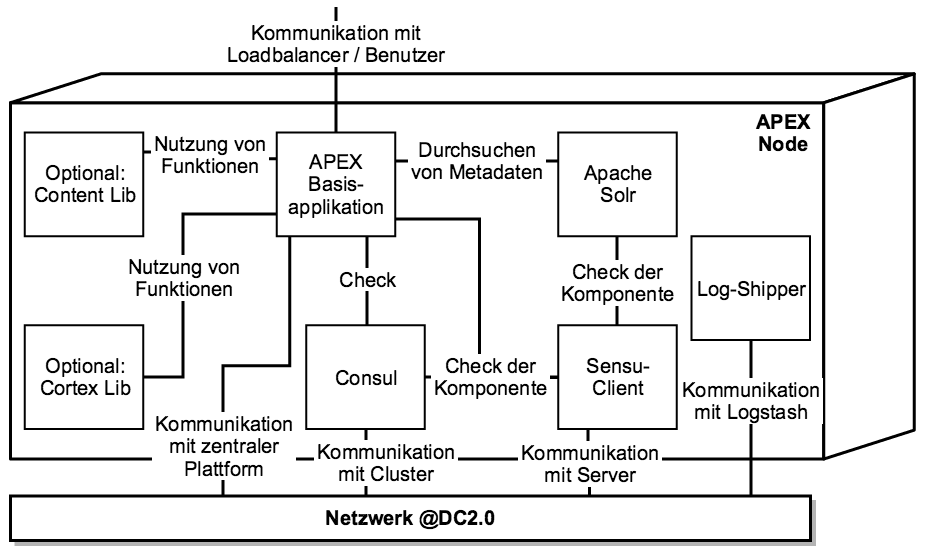
\includegraphics[width=0.7\textwidth]{img/apex.png}
	\caption[Minimaler Aufbau einer APEX Node]{Minimaler Aufbau einer APEX Node inklusive aller aktuell verfügbaren optionalen Bibliotheken}
	\label{fig:apex}
\end{figure} 
Wie bei den bisher beschriebenen Applikationen, sind außerdem noch Consul für die Kommunikation mit dem Loadbalancer und der Sensu-Client/Log-Shipper für die Integration in die Monitoring/Logging Infrastruktur vorhanden. Alle grundlegenden Komponenten des minimalen Aufbaus und ihre Abhängigkeiten untereinander, sind in \autoref{fig:apex} zu sehen. Zusätzlich zu den dargestellten Komponenten sind auch noch Java als Laufzeitumgebung und Supervisor für die Verwaltung der Komponenten installiert.

\paragraph{Automatisierung des Deployments:}
Bei der Automatisierung des Deployments muss nur APEX selbst, sowie der Apache Solr betrachtet werden. Für alle anderen Komponenten sind bereits Roles vorhanden, die wiederverwendet werden können. Die Automatisierung des Apache Solr stellte sich als unproblematisch heraus, da keine Abhängigkeiten bestehen und auch nicht auf Verteilungseigenschaften Rücksicht genommen werden musste. Eine größere Herausforderung stellt die Automatisierung von APEX selbst dar, da hierbei eine große Anzahl von Freiheitsgraden vorhanden ist. Außerdem kann nicht vorausgesagt werden, welche Komponenten die Stakeholder benötigen. Daher wurde das Deployment von APEX so generisch wie möglich gestaltet, um zukünftige Anforderungen der Stakeholder leicht unterstützen zu können.

Für das grundlegende Deployment von APEX konnte deswegen eine Role erstellt werden, bei dem aktuell bekannte Freiheitsgrade über Variablen gesteuert werden. Allerdings ist je Stakeholder ein eigenes Playbook notwendig, das diese APEX Role nutzt und zusätzlich den individuellen Code deployed. In diesem Playbook kann auch auf zusätzliche Komponenten Rücksicht genommen werden, die der Stakeholder benötigt. In diesem Fall ist es also nicht möglich, für jeden Stakeholder dieselben Ansible Playbooks wiederzuverwenden. Man kann lediglich das Grundgerüst der Komponenten automatisieren, es wird aber für jeden neuen Stakeholder ein erneuter initialer Aufwand notwendig sein.

\paragraph{Erfassen der Metriken:}
Bei dem APEX Framework handelt es sich um eine Neuentwicklung, weswegen kein Vergleich zum DC1.0 aufgestellt werden kann. 

Die Anzahl der Komponenten bezieht sich auf das Grundgerüst von APEX, mit der Basisapplikation und dem Apache Solr. Es wurde keine spezifische Komponente eines Stakeholders mit einbezogen. Aus diesem Grund ist der initiale Aufwand auch geteilt. Die erste Zahl in \autoref{tab:metric:apex} bezieht sich auf den Aufwand der Implementierung für das Grundgerüst von APEX. Dieser Aufwand ist nur einmal notwendig und unabhängig von der Anzahl der Stakeholder. Die zweite Zahl bezieht sich auf den einmaligen Aufwand, der für jeden weiteren Stakeholder nötig ist, um APEX vorzubereiten. Zusätzlich kommt noch der Aufwand für die Automatisierung spezieller Komponenten, die der Stakeholder benötigt dazu. Diese können aber im Voraus nicht abgeschätzt werden.

Die Basisapplikation von APEX ist zustandslos und kann verteilt betrieben werden. Da die Möglichkeit der Verteilung grundlegend vom individuellen Code des Stakeholders abhängt, wird APEX in diesem Fall nicht als verteilte Applikation betrachtet. Dies wird voraussichtlich auch den Hauptanwendungsfall von APEX ausmachen. 

\begin{table}[ht]
%\setlength{\arrayrulewidth}{0.3mm}
\setlength{\tabcolsep}{5pt}
\renewcommand{\arraystretch}{1.5}
\centering
\begin{tabular}{|l|l|l|}
\hline
\rowcolor[HTML]{C0C0C0}
\multicolumn{2}{|c|}{\textbf{Metrik}} & \textbf{Menge}					\\ 
\hline
\multirow{3}{*}{Initialer Aufwand}	& Implementation & 100 PS	\\ 
\cline{2-3}
									& je Stakeholder & 8 PS \\
\cline{2-3}
									& wiederverwendete Roles & 5		\\
\hline 
\multirow{2}{*}{Komplexität}			& Anzahl der Komponenten & 7		\\
\cline{2-3}
									& verteiltes System		& Nein 		\\
\hline
\multirow{3}{*}{Durchlaufzeit} & a.) eine Node		& ca. 4 Minuten	\\ 
\cline{2-3} 
									& b.) alle Nodes		& ca. 4 Minuten	\\ 
\cline{2-3}							
									& c.) zusätzliche Node	& ca. 8 Minuten \\
\hline
\end{tabular} 
\caption{Erfasste Metriken des APEX Frameworks}
\label{tab:metric:apex}
\end{table}

Da es, je Ausprägung von APEX, nur eine Node geben wird, ist die Zeit für alle Nodes gleich der Zeit für eine Node. Ein Deployment auf allen Nodes macht in diesem Fall keinen Sinn und müsste auch mit allen Stakeholdern abgesprochen werden. Dies wäre nur der Fall, wenn sich kritische Änderungen am Grundgerüst ergeben, die sofort auf allen Nodes ausgerollt werden müssen. Dann müsste man die Zeit für eine Node, lediglich mit der Anzahl der Nodes multiplizieren, um die gesamt benötigte Zeit für ein sequentielles Update zu erhalten.
